\begin{figure}[!ht]
\settoheight{\tempdima}{\includegraphics[width=.3\linewidth]{example-image-a}}%
\centering\begin{tabular}{@{}c@{ }c@{ }c@{ }c@{}}
&\textbf{Hornet} & \textbf{Gunrock} & \textbf{cuGraph} \\
\rowname{\small\textbf{BFS}}
&
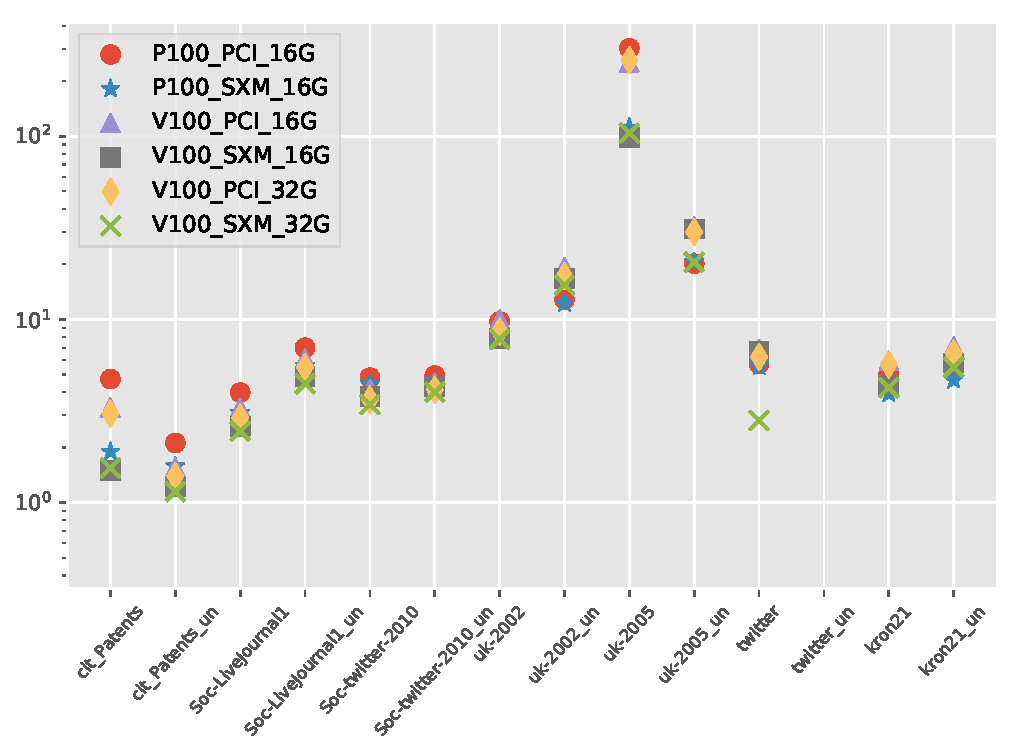
\includegraphics[width=.32\linewidth]{plots/log_GTEPS_G_BFS_Hornet.pdf}&
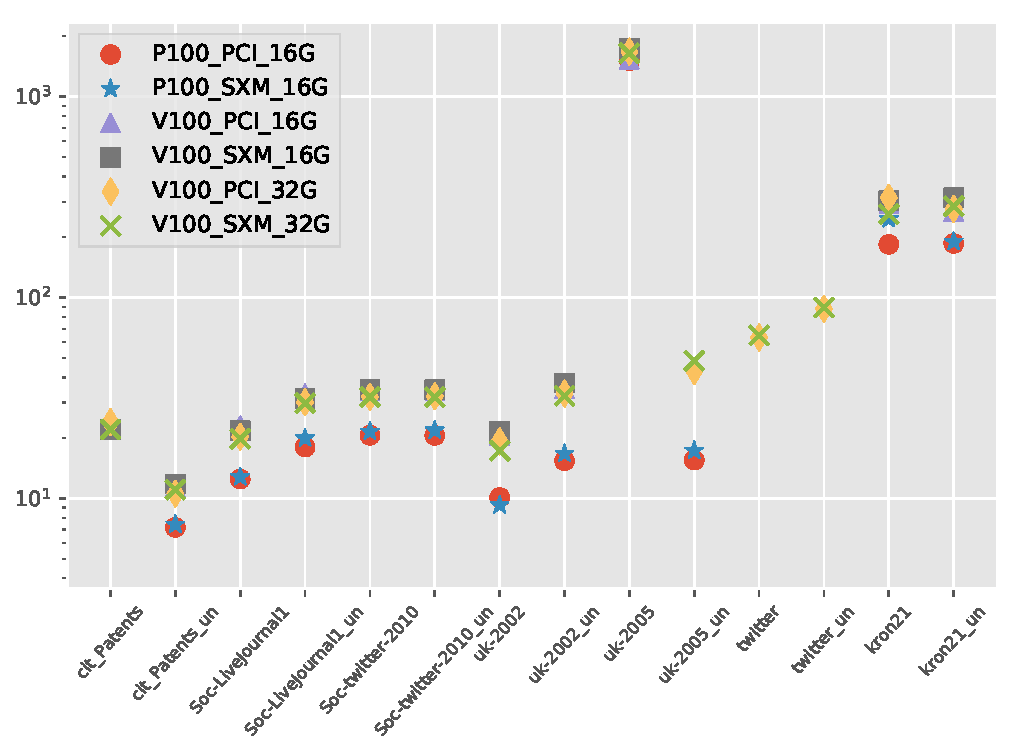
\includegraphics[width=.32\linewidth]{plots/log_GTEPS_G_BFS_Gunrock_Opt.pdf}&
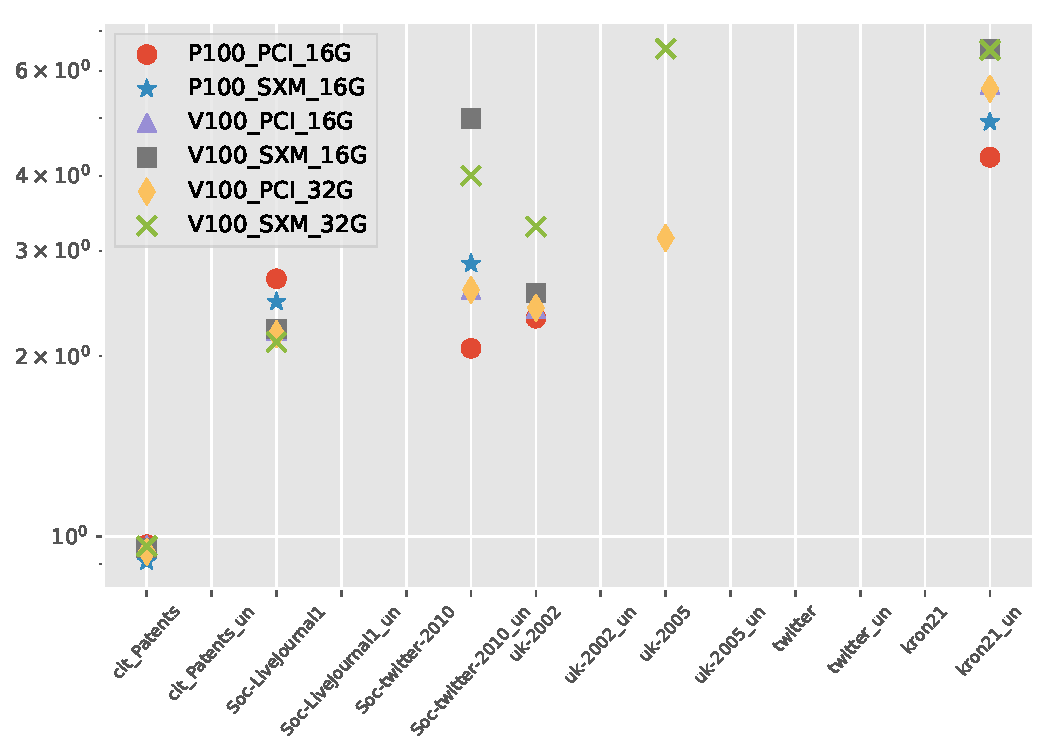
\includegraphics[width=.32\linewidth]{plots/log_GTEPS_G_BFS_cuGraph.pdf}\\[-1ex]
%&\mycaption{0.2} & \mycaption{0.2} & \mycaption{0.3}\\
\rowname{\small\textbf{PR}}
&
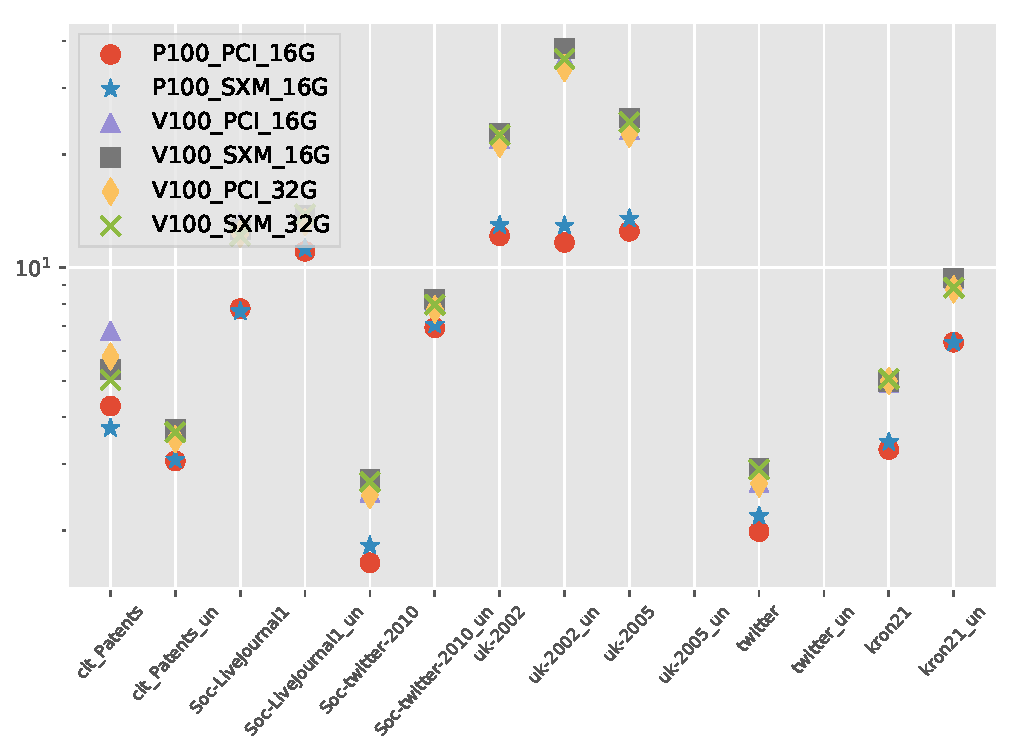
\includegraphics[width=.32\linewidth]{plots/log_GTEPS_G_PR_Hornet.pdf}&
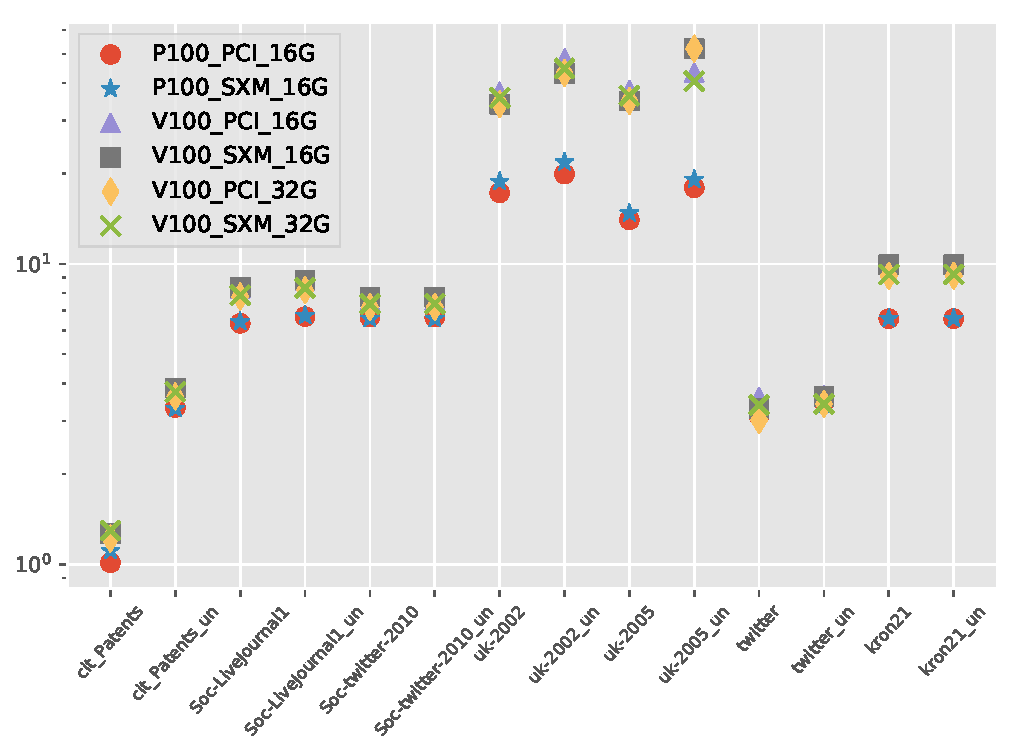
\includegraphics[width=.32\linewidth]{plots/log_GTEPS_G_PR_Gunrock_Opt.pdf}&
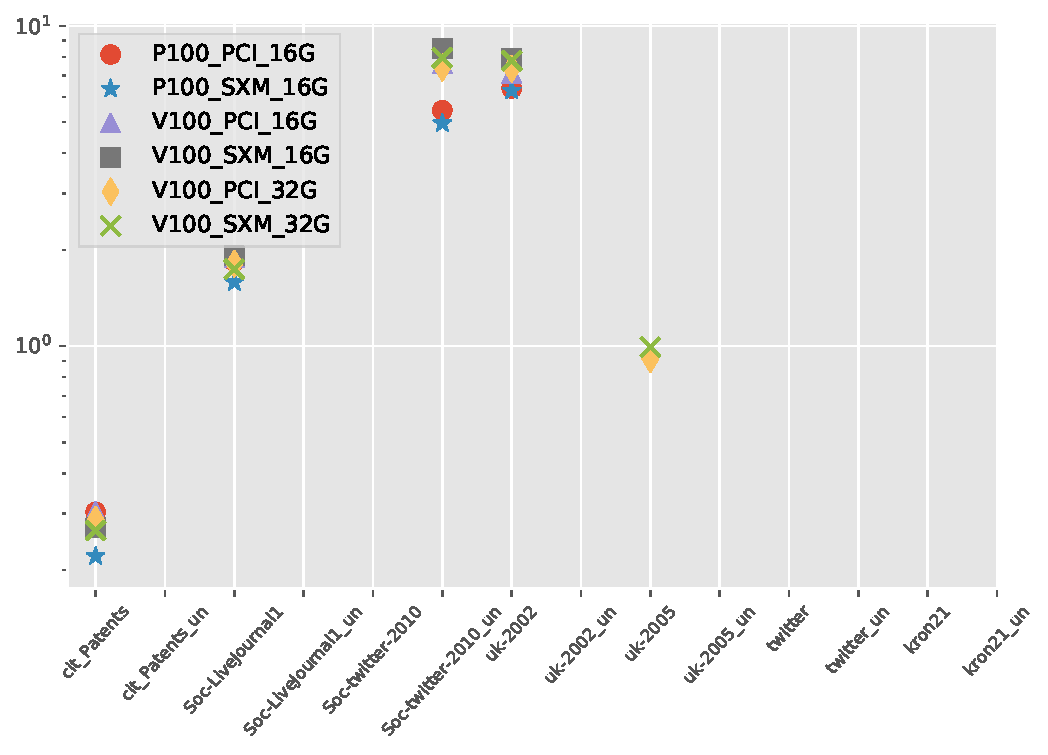
\includegraphics[width=.32\linewidth]{plots/log_GTEPS_G_PR_cuGraph.pdf}\\[-1ex]
%&\mycaption{0.5} & \mycaption{0.4} & \mycaption{0.6}%\\
\rowname{\small\textbf{BC}}&
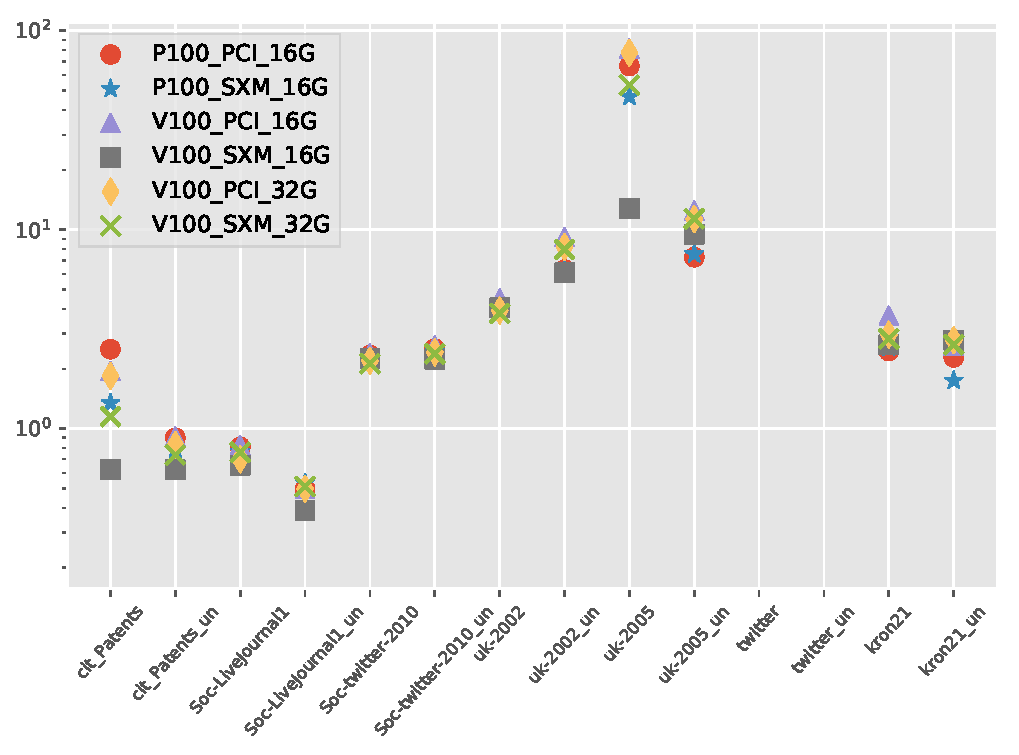
\includegraphics[width=.32\linewidth]{plots/log_GTEPS_G_BC_Hornet.pdf}&
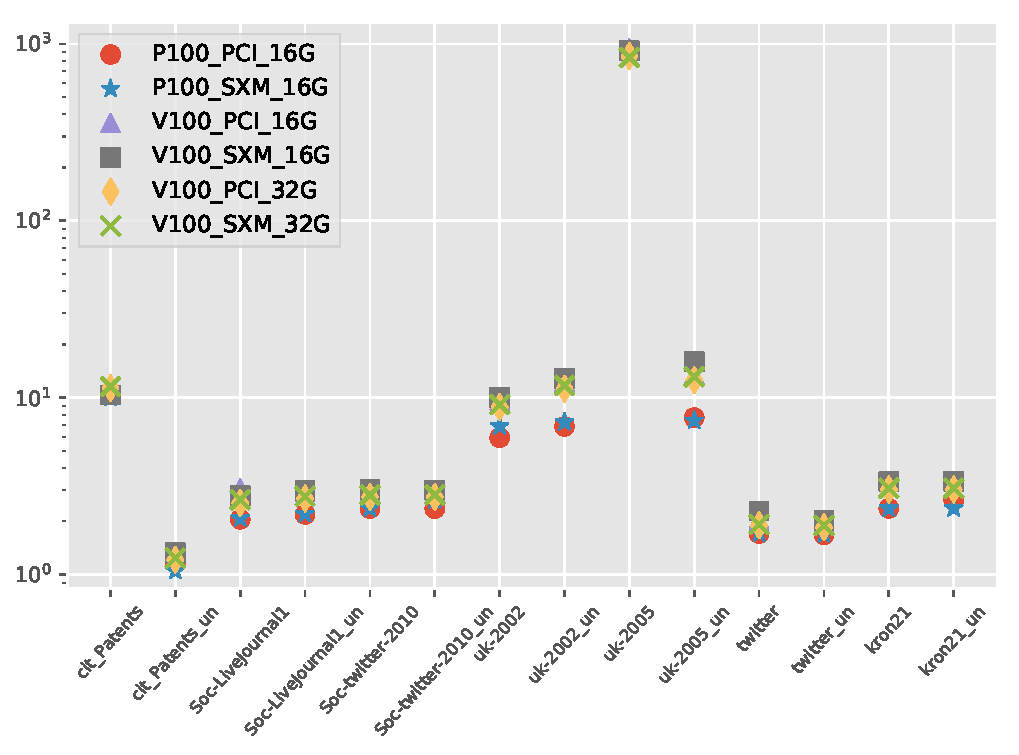
\includegraphics[width=.32\linewidth]{plots/log_GTEPS_G_BC_Gunrock_Opt.pdf}&
\includegraphics[width=.32\linewidth]{}\\[-1ex]
%&\mycaption{0.5} & \mycaption{0.4} & \mycaption{0.6}%\\
\rowname{\small\textbf{CC}}&
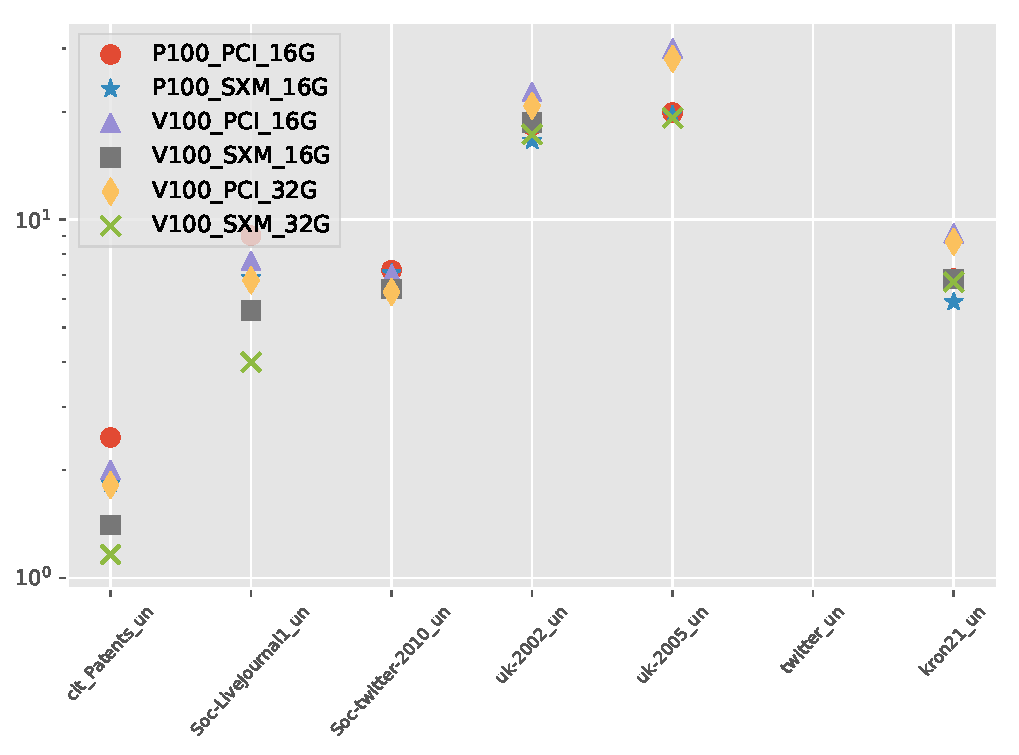
\includegraphics[width=.32\linewidth]{plots/log_GTEPS_G_CC_Hornet.pdf}&
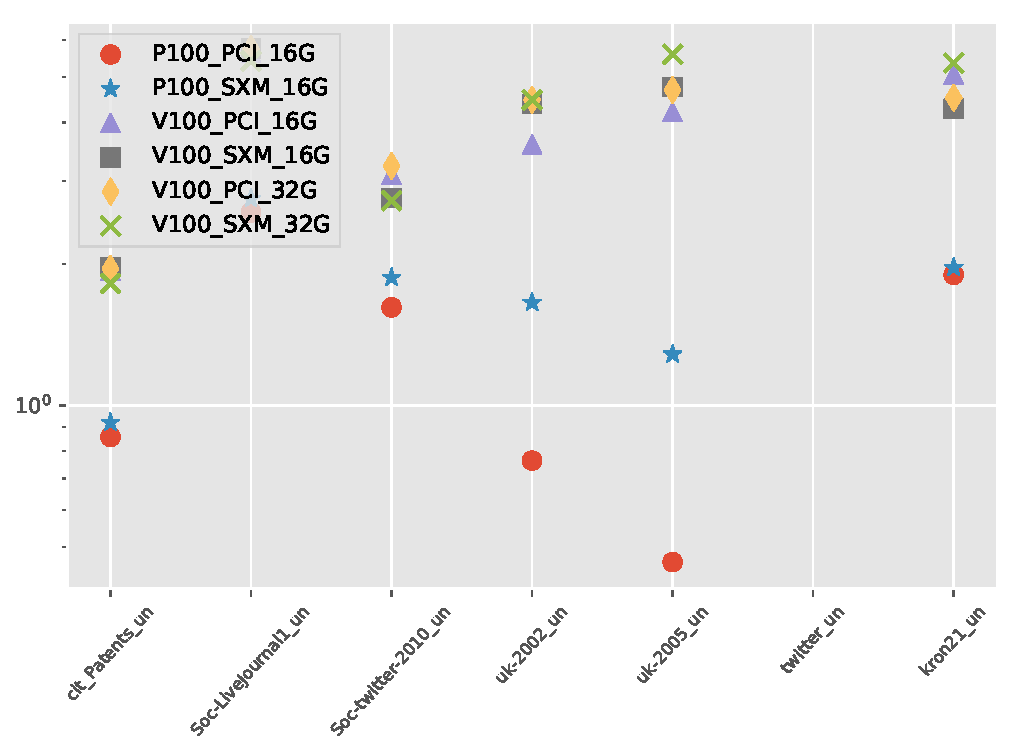
\includegraphics[width=.32\linewidth]{plots/log_GTEPS_G_CC_Gunrock_Def.pdf}&
\includegraphics[width=.23\linewidth]{}\\[-1ex]
%&\mycaption{0.5} & \mycaption{0.4} & \mycaption{0.6}%\\
\rowname{\small\textbf{TC}}&
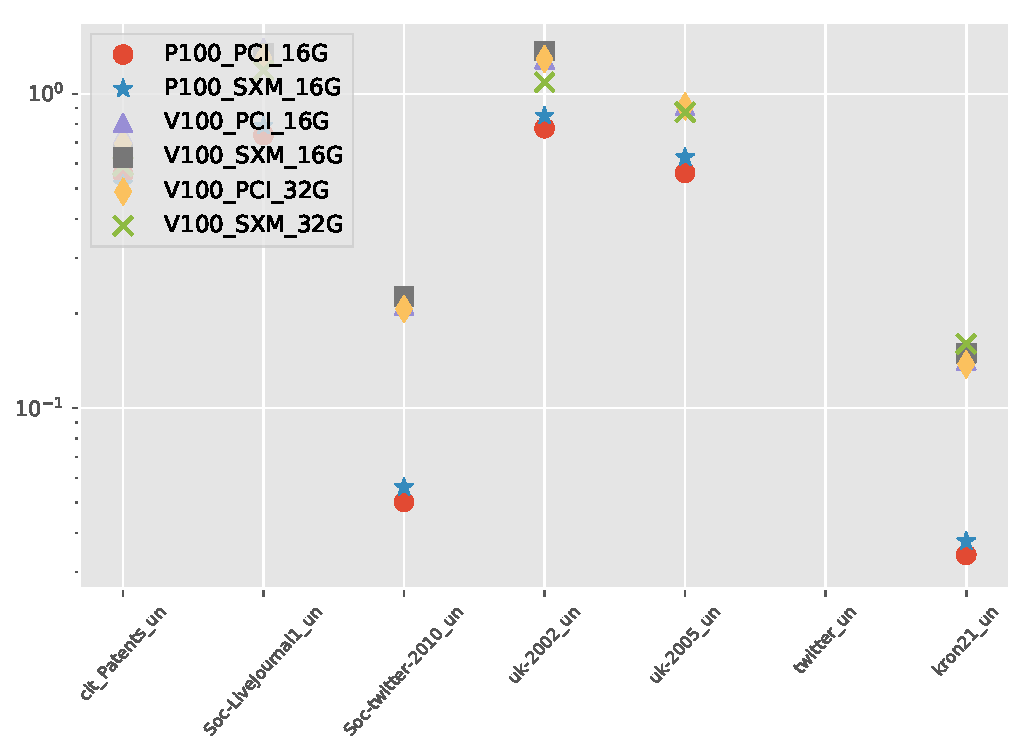
\includegraphics[width=.32\linewidth]{plots/log_GTEPS_G_TC_Hornet.pdf}&
\includegraphics[width=.32 \linewidth]{}&
\includegraphics[width=.32 \linewidth]{}\\[-1ex]
%&\mycaption{0.5} & \mycaption{0.4} & \mycaption{0.6}%\\
\end{tabular}
\caption{Logarithmic GTEPS of each benchmark with real world and synthetic graph(s) in Hornet, Gunrock, and cuGraph}%
\label{figure1}
\end{figure}

\begin{figure}
\settoheight{\tempdima}{\includegraphics[width=.3\linewidth]{example-image-a}}%
\centering\begin{tabular}{@{}c@{ }c@{ }c@{ }}
&\textbf{PCI} & \textbf{SXM} &
\rowname{(P100-16GB) \small\textbf{BFS}}&
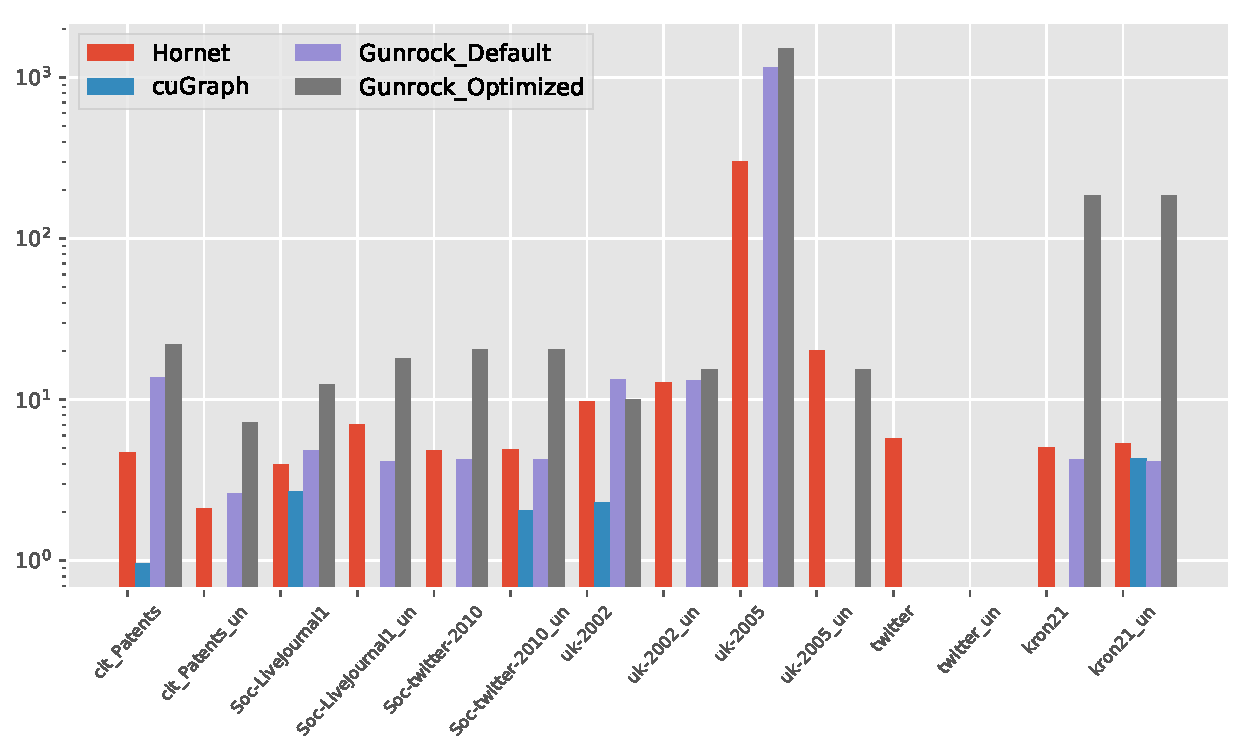
\includegraphics[width=.45\linewidth]{plots/log_GTEPS_G_BFS_PP16.pdf}&
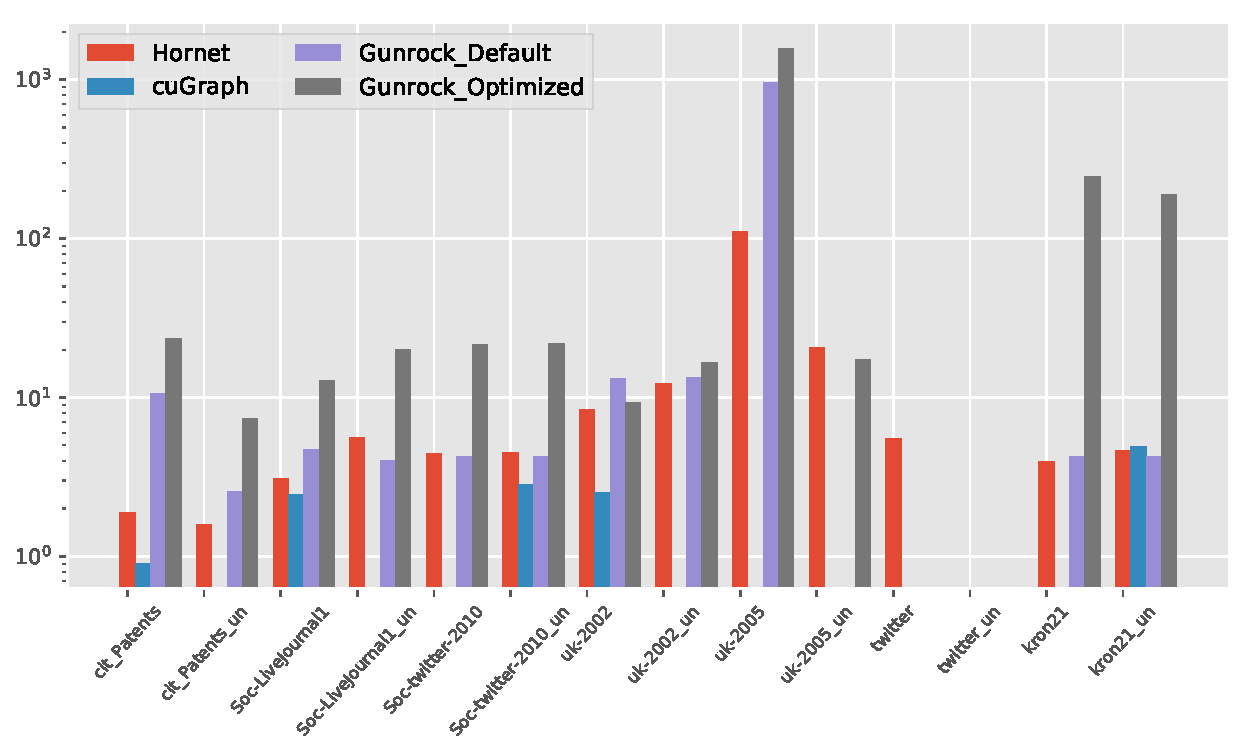
\includegraphics[width=.45\linewidth]{plots/log_GTEPS_G_BFS_PS16.pdf}\\[-1ex]
\rowname{(V100-16GB) \small\textbf{BFS}}&
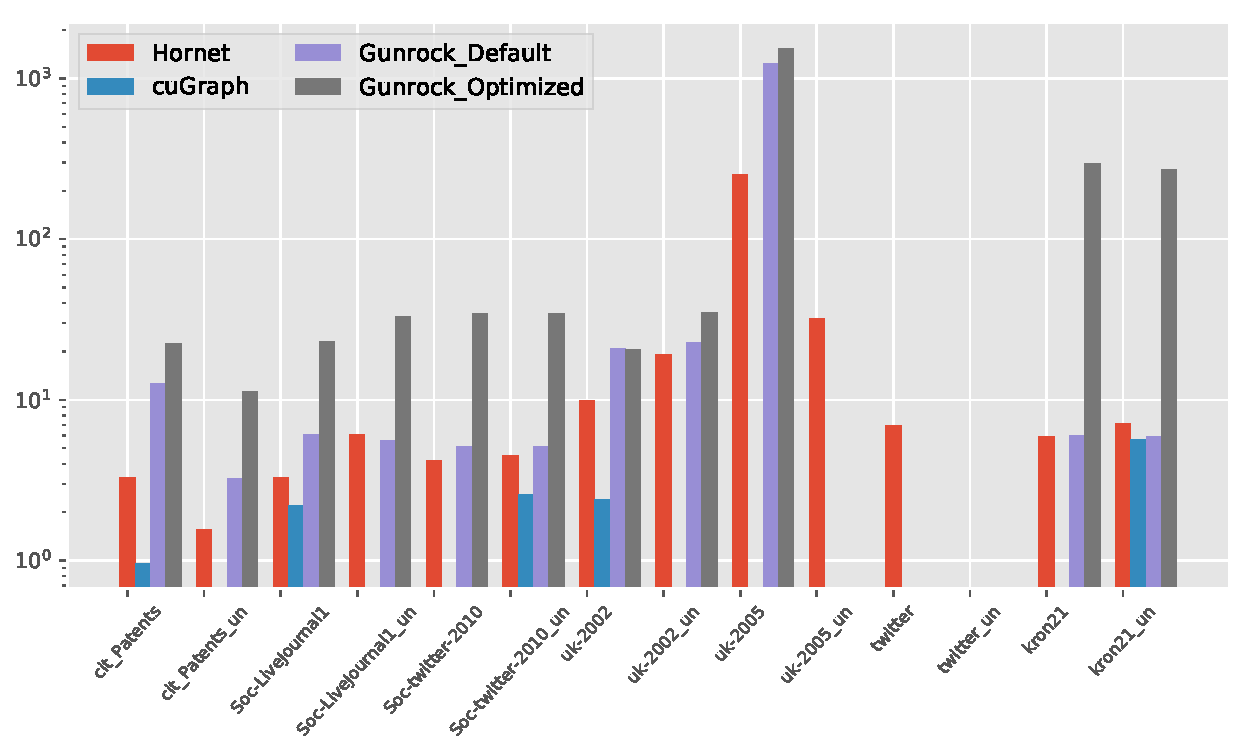
\includegraphics[width=.45\linewidth]{plots/log_GTEPS_G_BFS_VP16.pdf}&
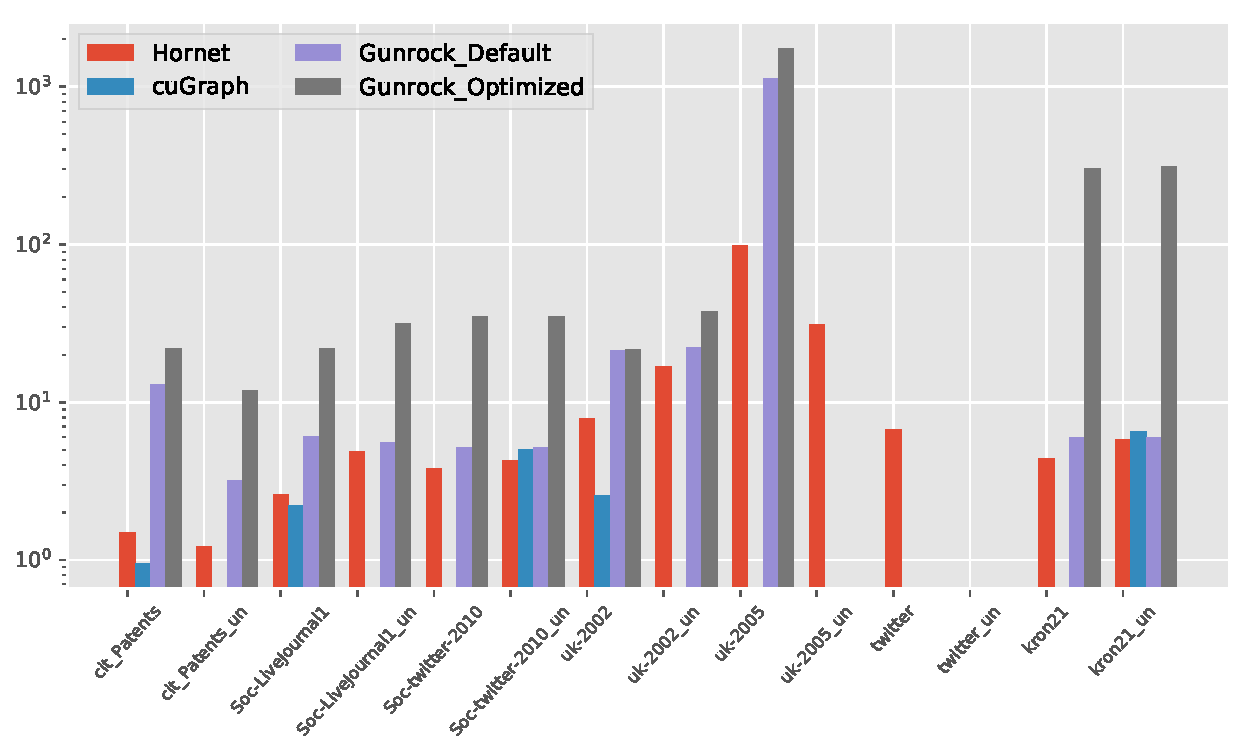
\includegraphics[width=.45\linewidth]{plots/log_GTEPS_G_BFS_VS16.pdf}\\[-1ex]
\rowname{(V100-32GB) \small\textbf{BFS}}&
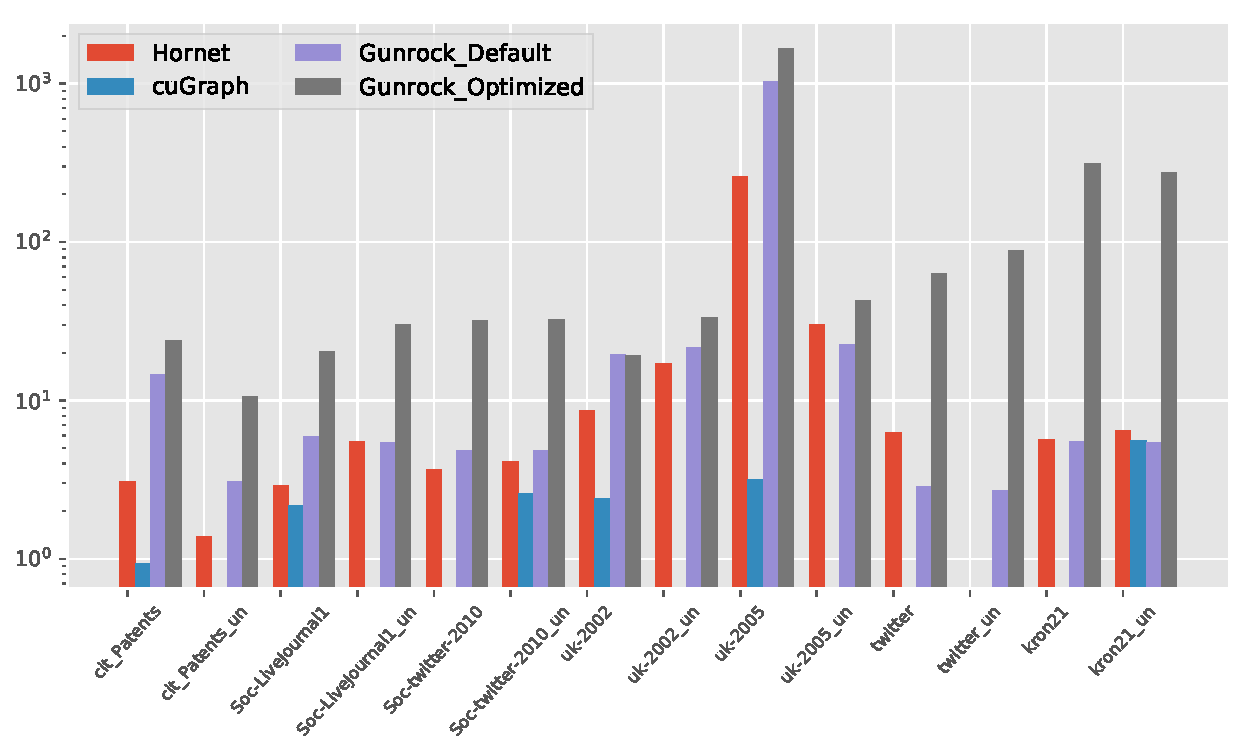
\includegraphics[width=.45\linewidth]{plots/log_GTEPS_G_BFS_VP32.pdf}&
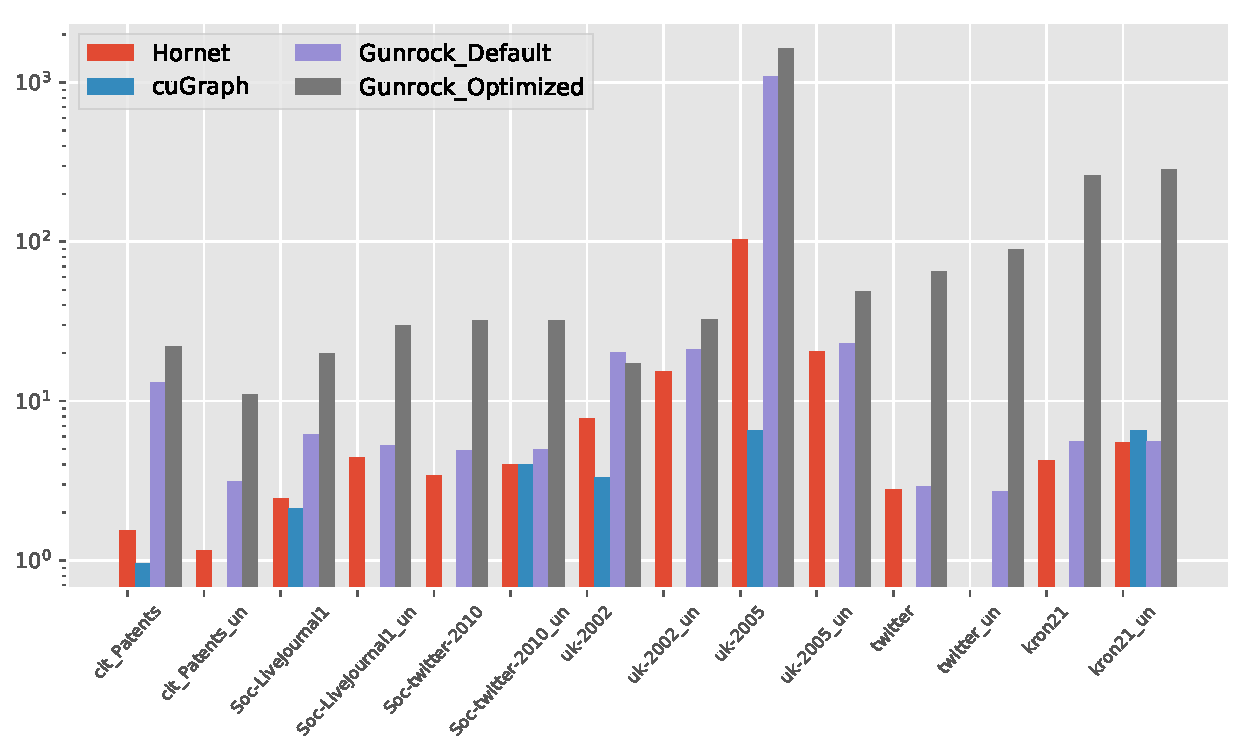
\includegraphics[width=.45\linewidth]{plots/log_GTEPS_G_BFS_VS32.pdf}\\[-1ex]
\rowname{(P100-16GB) \small\textbf{PR}}&
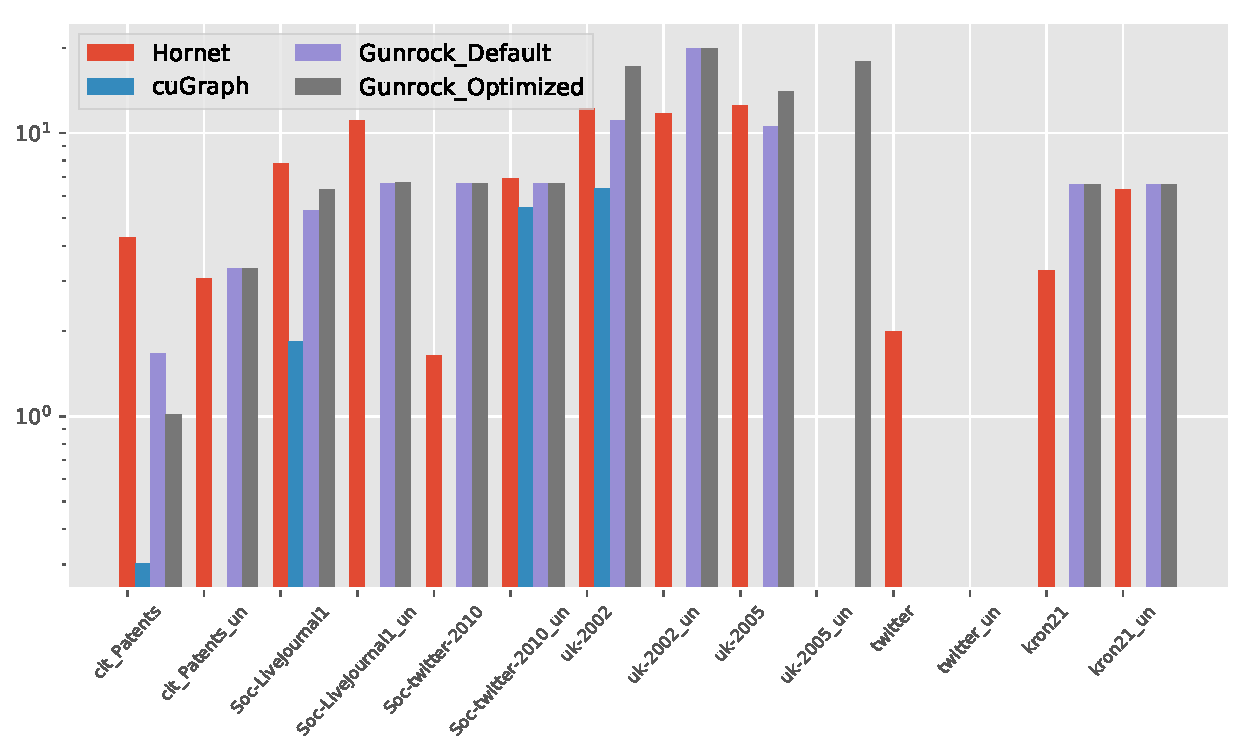
\includegraphics[width=.45\linewidth]{plots/log_GTEPS_G_PR_PP16.pdf}&
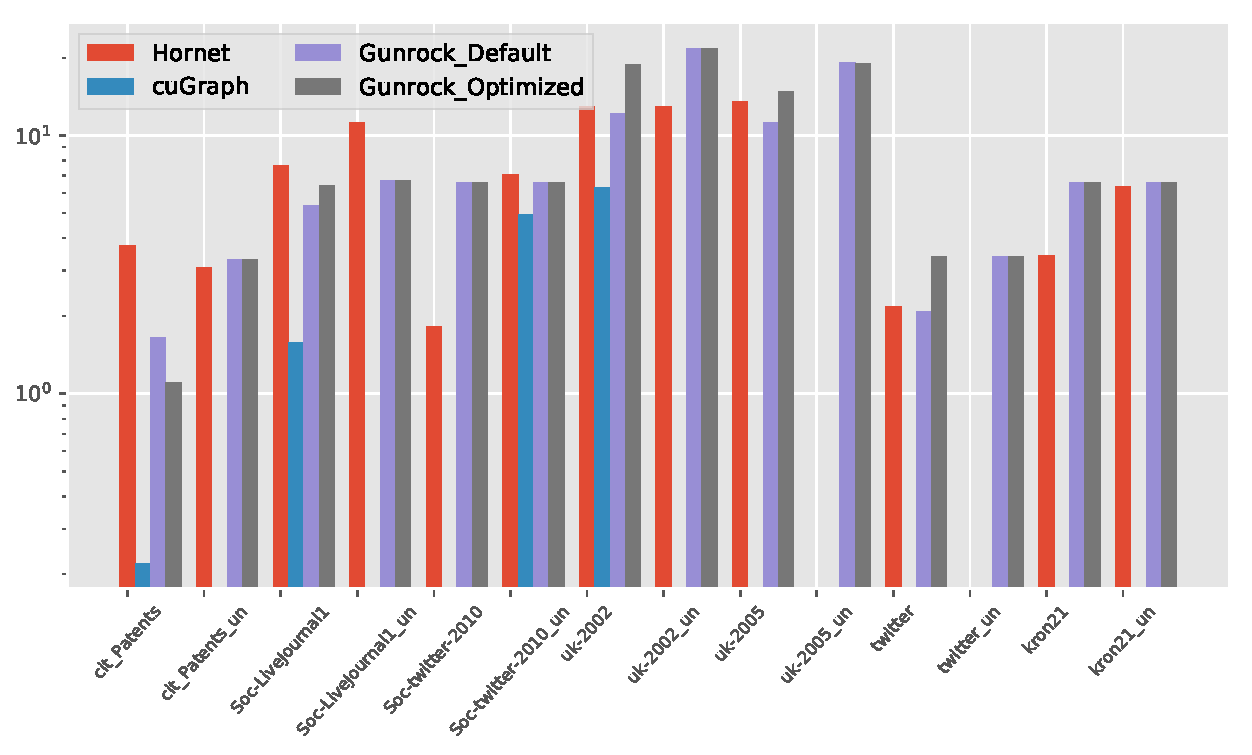
\includegraphics[width=.45\linewidth]{plots/log_GTEPS_G_PR_PS16.pdf}\\[-1ex]
\rowname{(V100-16GB) \small\textbf{PR}}&
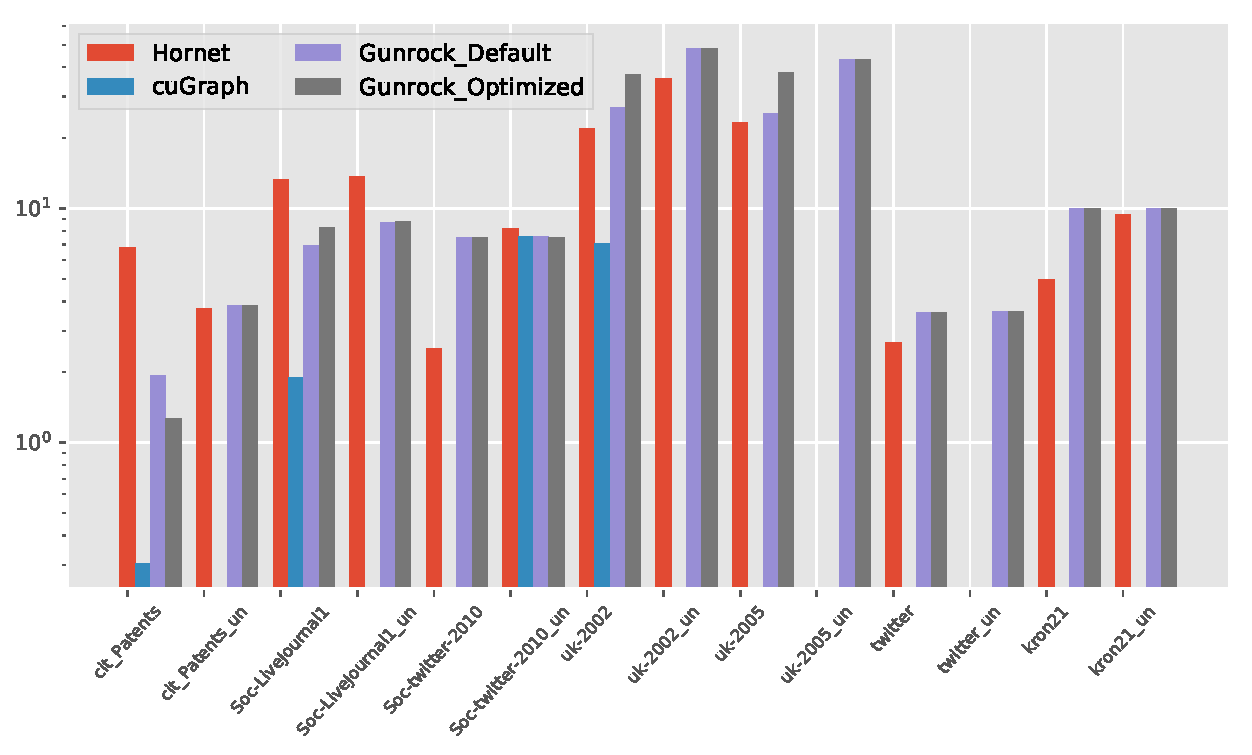
\includegraphics[width=.45\linewidth]{plots/log_GTEPS_G_PR_VP16.pdf}&
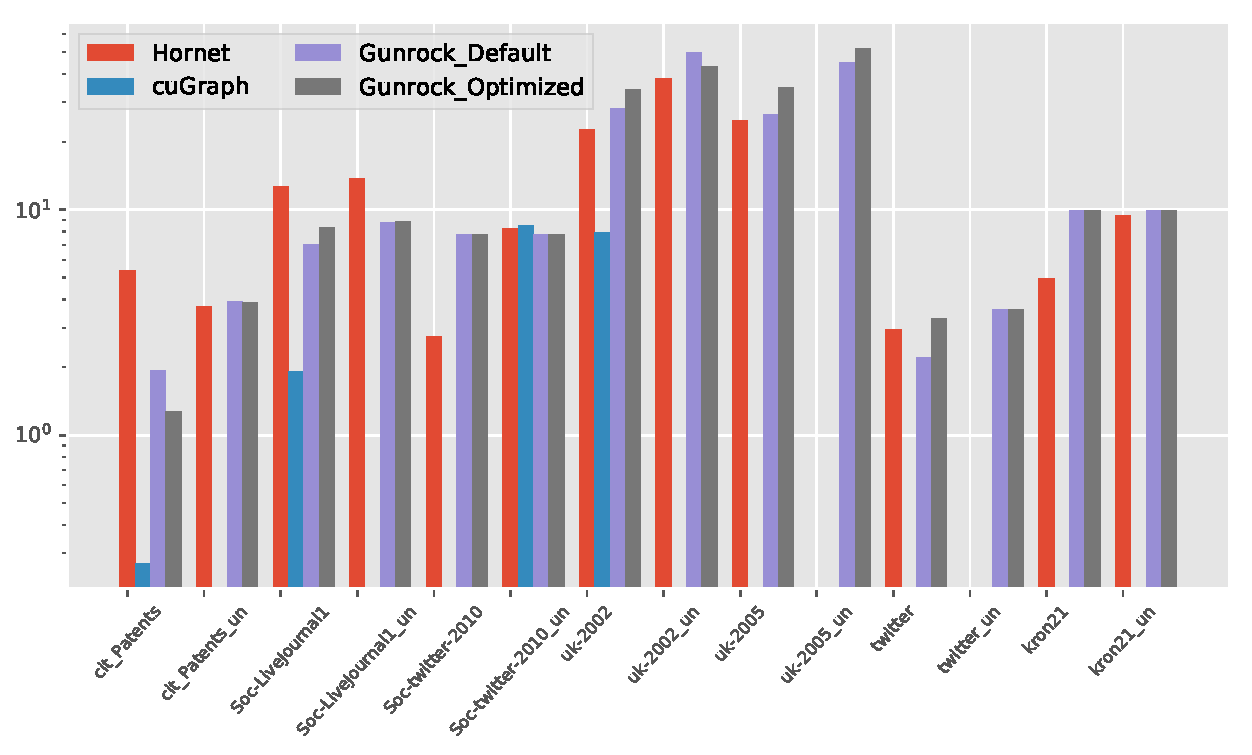
\includegraphics[width=.45\linewidth]{plots/log_GTEPS_G_PR_VS16.pdf}\\[-1ex]
\rowname{(V100-32GB) \small\textbf{PR}}&
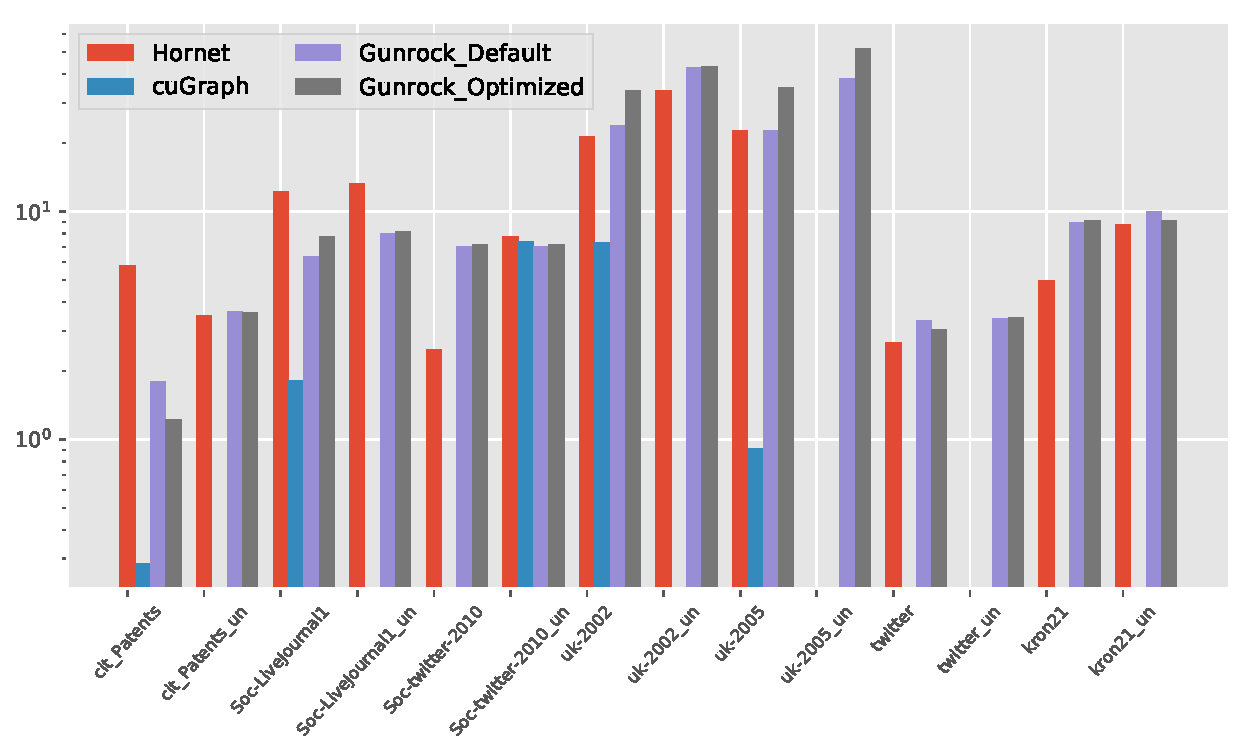
\includegraphics[width=.45\linewidth]{plots/log_GTEPS_G_PR_VP32.pdf}&
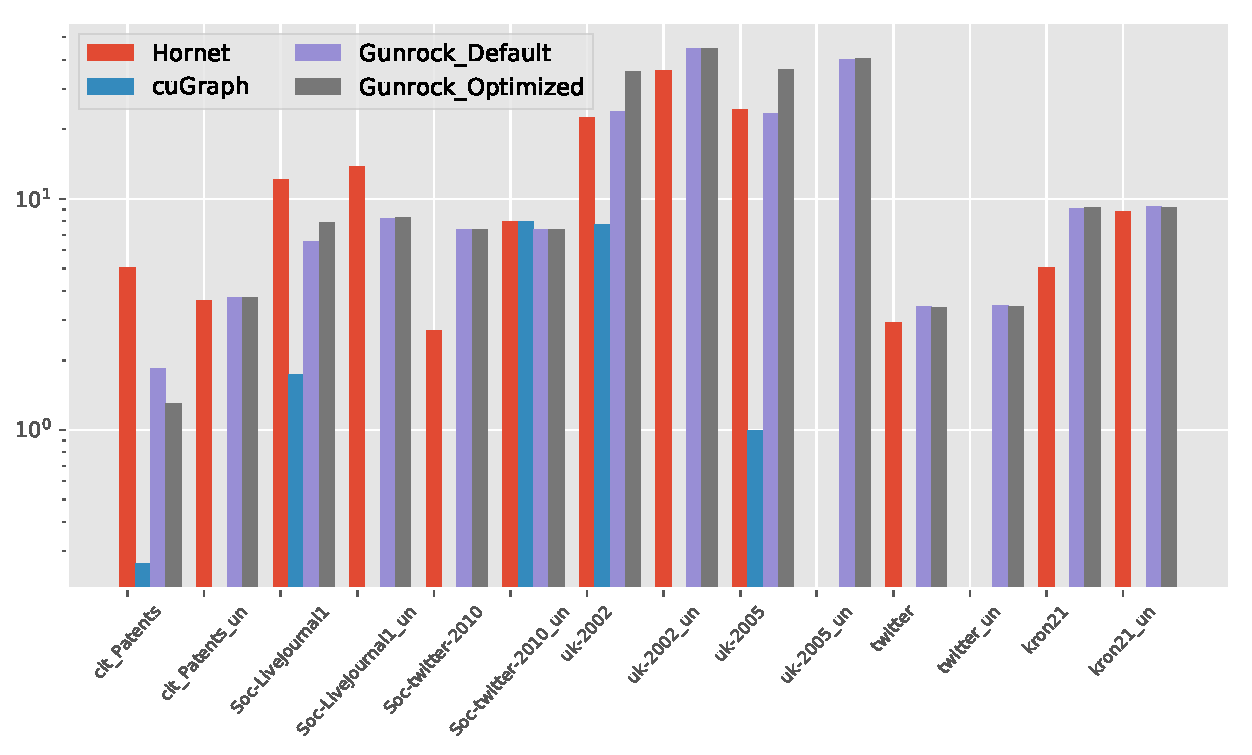
\includegraphics[width=.45\linewidth]{plots/log_GTEPS_G_PR_VS32.pdf}\\[-1ex]
\rowname{(P100-16GB) \small\textbf{BC}}&
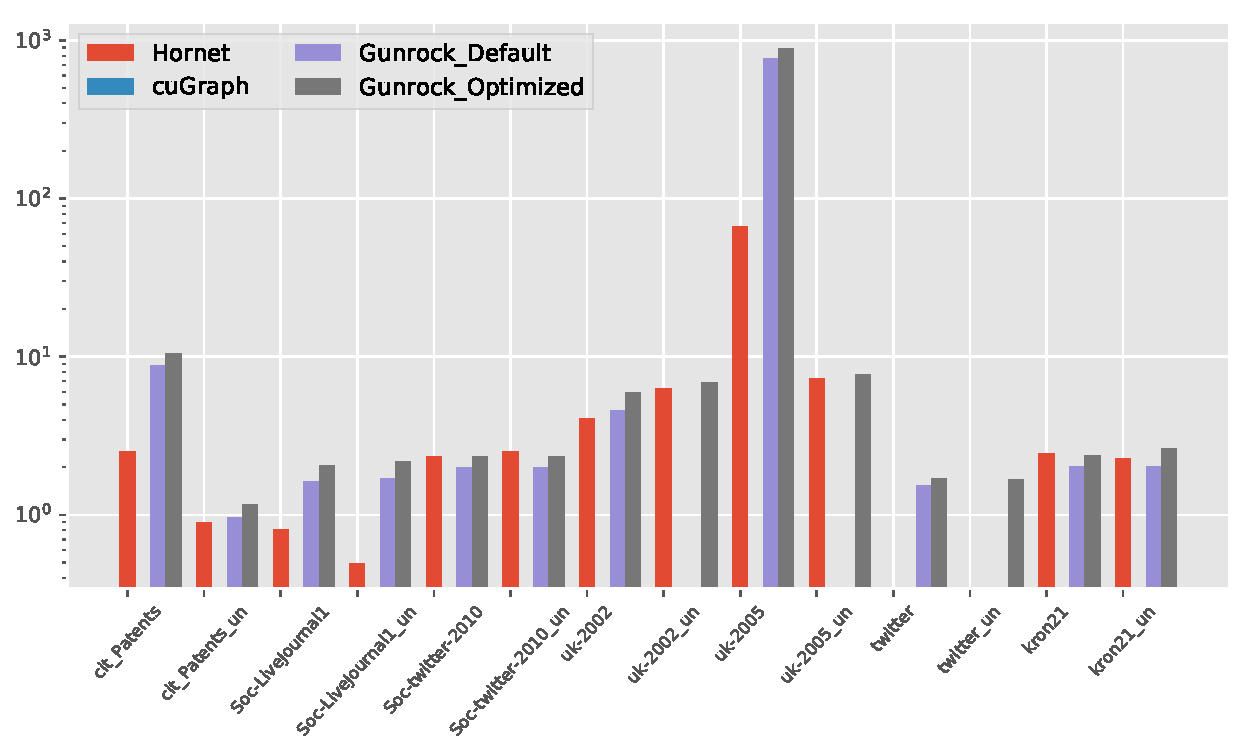
\includegraphics[width=.45\linewidth]{plots/log_GTEPS_G_BC_PP16.pdf}&
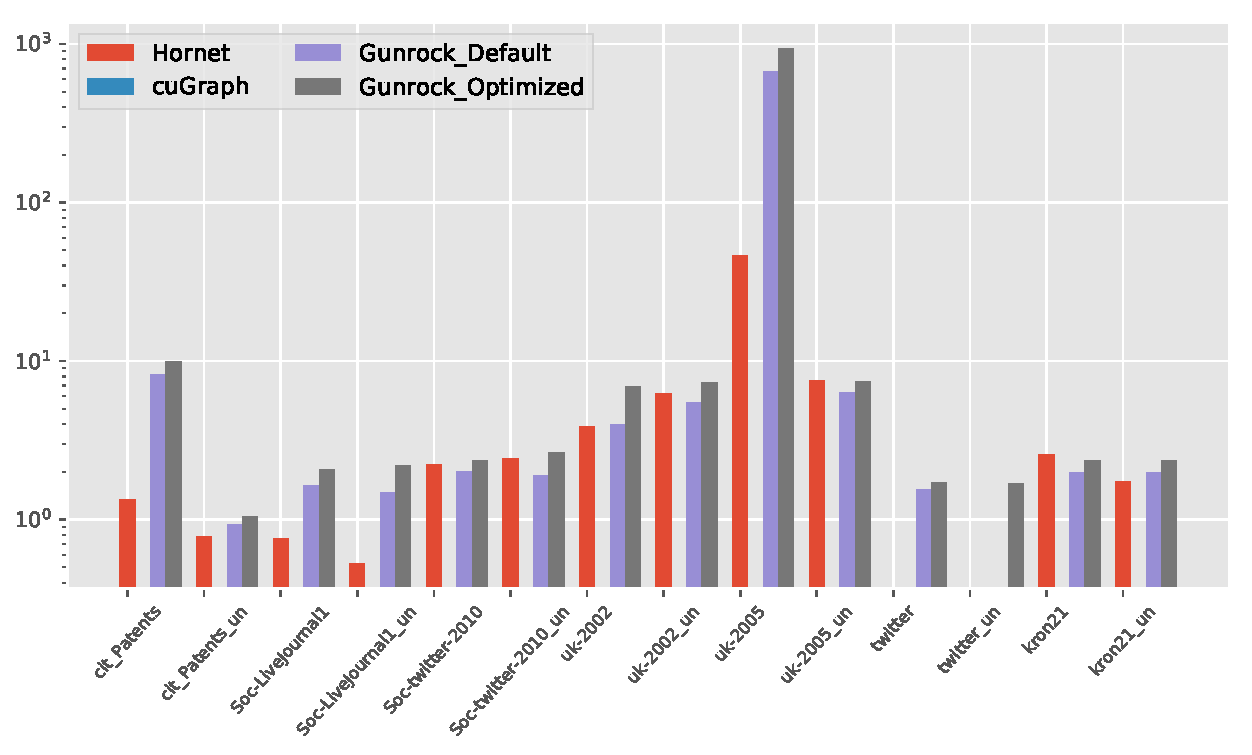
\includegraphics[width=.45\linewidth]{plots/log_GTEPS_G_BC_PS16.pdf}\\[-1ex]
\rowname{(V100-16GB) \small\textbf{BC}}&
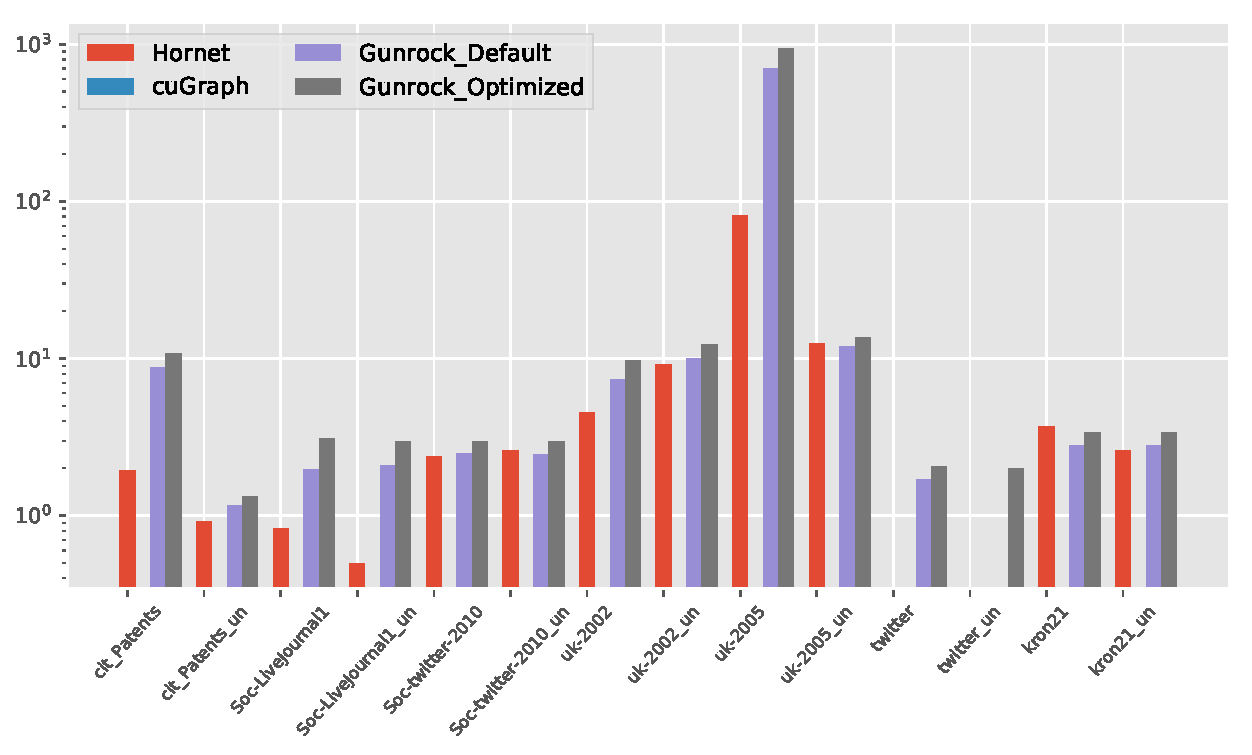
\includegraphics[width=.45\linewidth]{plots/log_GTEPS_G_BC_VP16.pdf}&
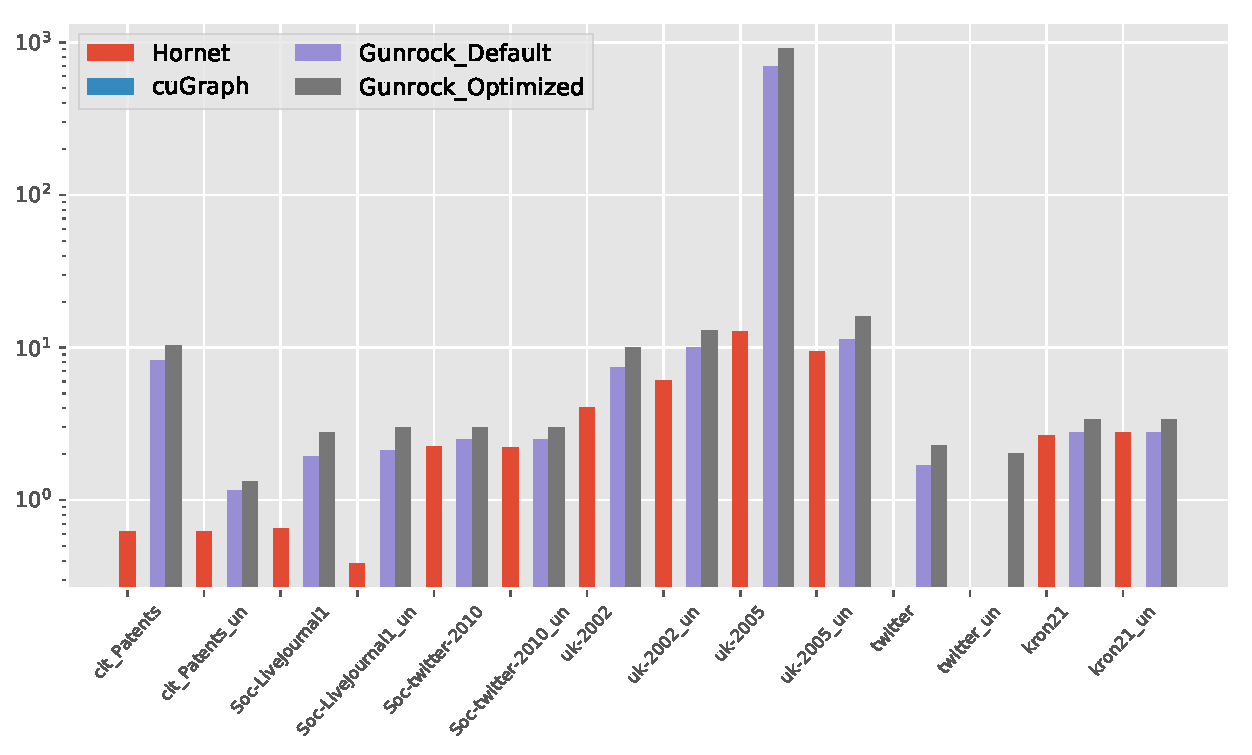
\includegraphics[width=.45\linewidth]{plots/log_GTEPS_G_BC_VS16.pdf}\\[-1ex]
\rowname{(V100-32GB) \small\textbf{BC}}&
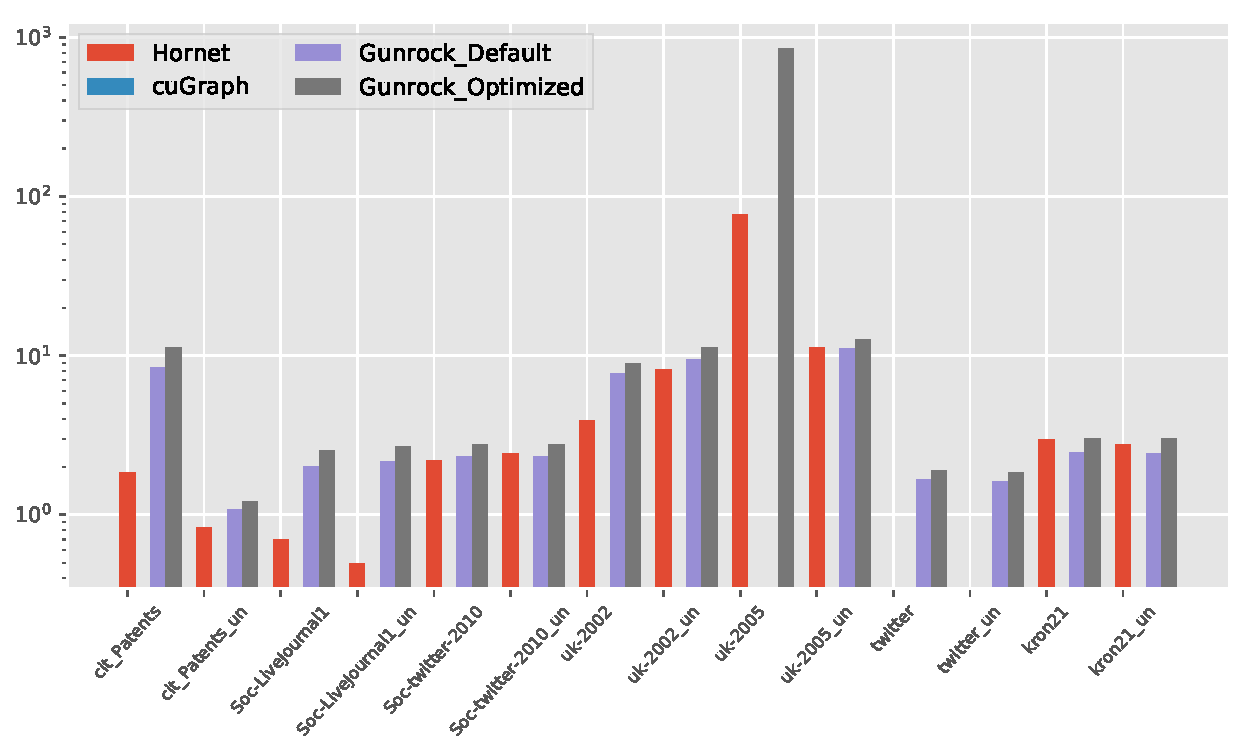
\includegraphics[width=.45\linewidth]{plots/log_GTEPS_G_BC_VP32.pdf}&
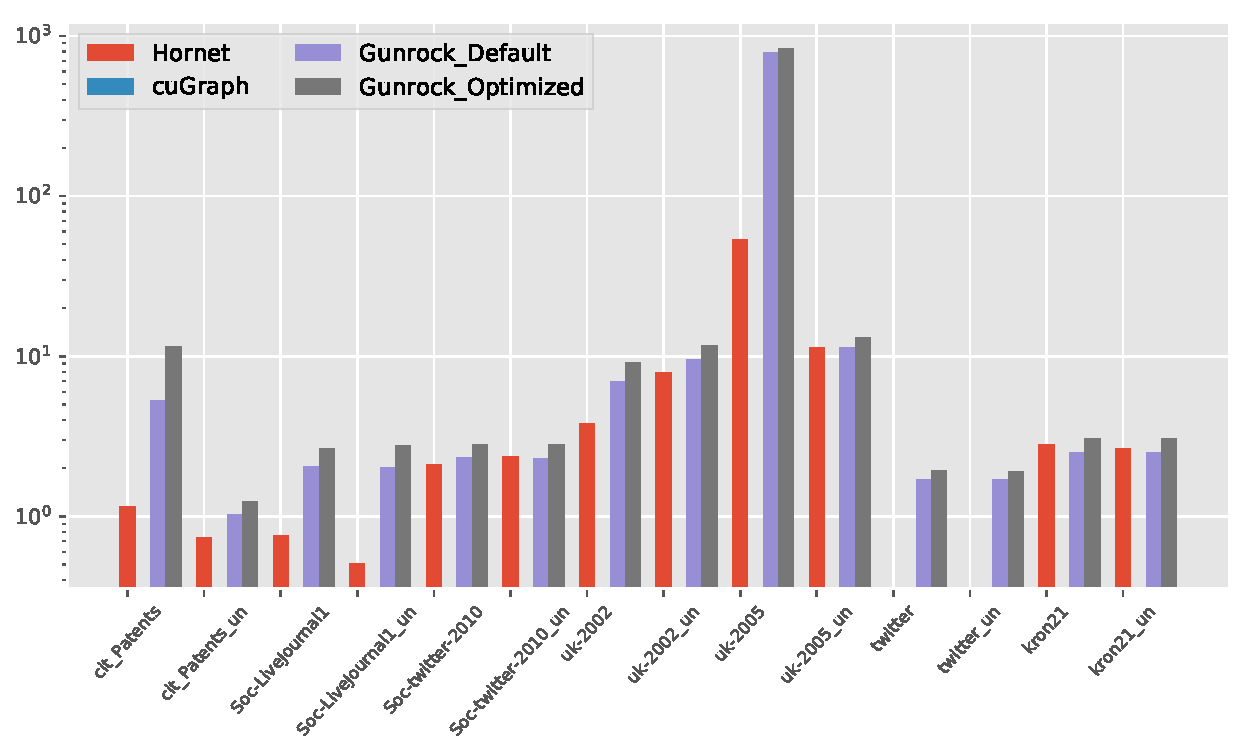
\includegraphics[width=.45\linewidth]{plots/log_GTEPS_G_BC_VS32.pdf}\\[-1ex]
\end{tabular}
\caption{GTEPS of benchmarks BFS, PR, BC, CC, and TC in six different GPU systems. Traveral algorithms such as BFS are executed with the largest degree node as a root. Some benchmarks are available in all frameworks, such as CC in cuGraph. A few computations are not completed and not shown to OOM(Out-of-memory)}%
\label{fig:GTEPS_ALL}
\end{figure}

\begin{figure}
\settoheight{\tempdima}{\includegraphics[width=.3\linewidth]{example-image-a}}%
\centering\begin{tabular}{@{}c@{ }c@{ }c@{ }} 
& \textbf{PCI} & \textbf{SXM} &
\rowname{(P100-16GB) \small\textbf{CC}}&
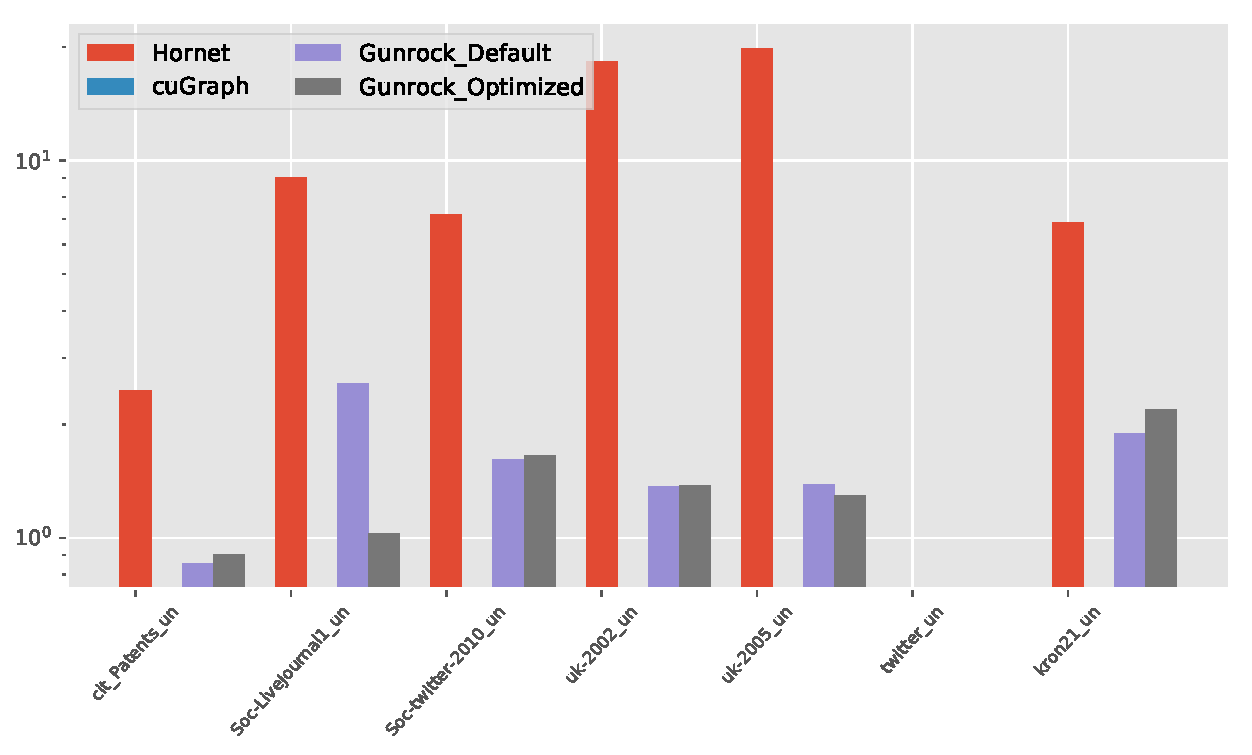
\includegraphics[width=.4\linewidth]{plots/log_GTEPS_G_CC_PP16.pdf}&
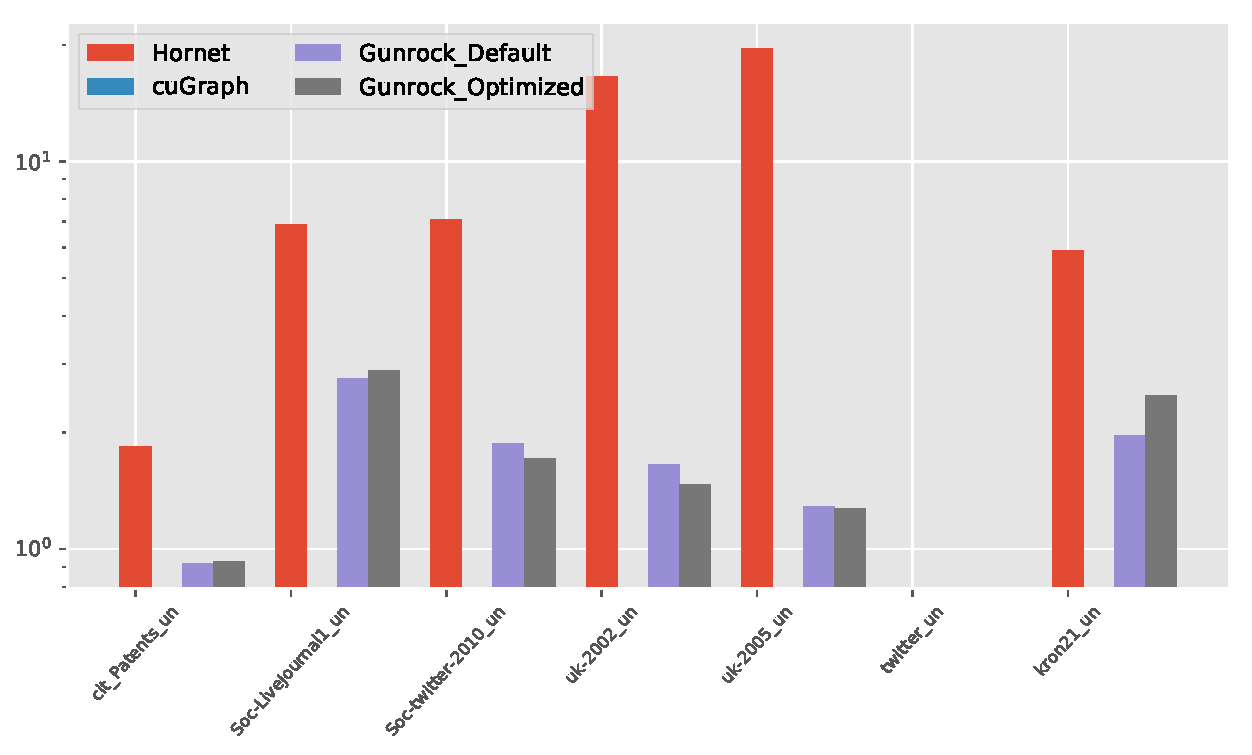
\includegraphics[width=.4\linewidth]{plots/log_GTEPS_G_CC_PS16.pdf}\\[-1ex]
\rowname{(V100-16GB) \small\textbf{CC}}&
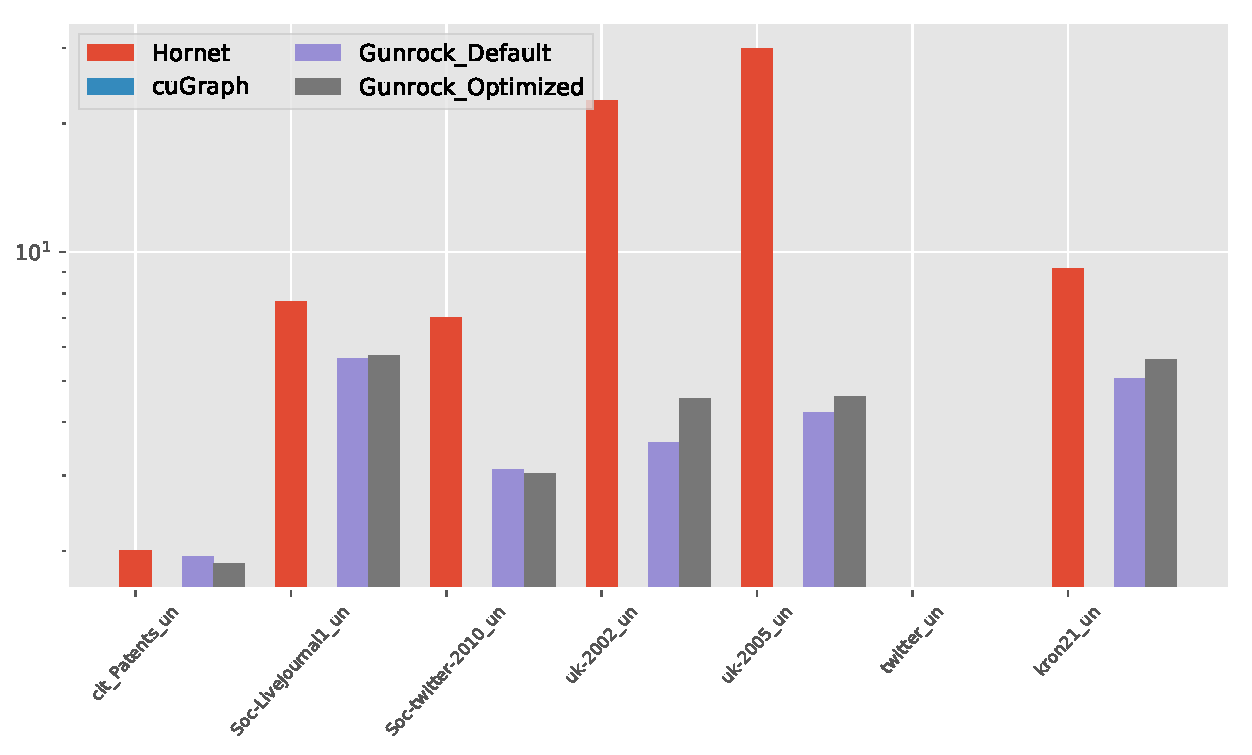
\includegraphics[width=.4\linewidth]{plots/log_GTEPS_G_CC_VP16.pdf}&
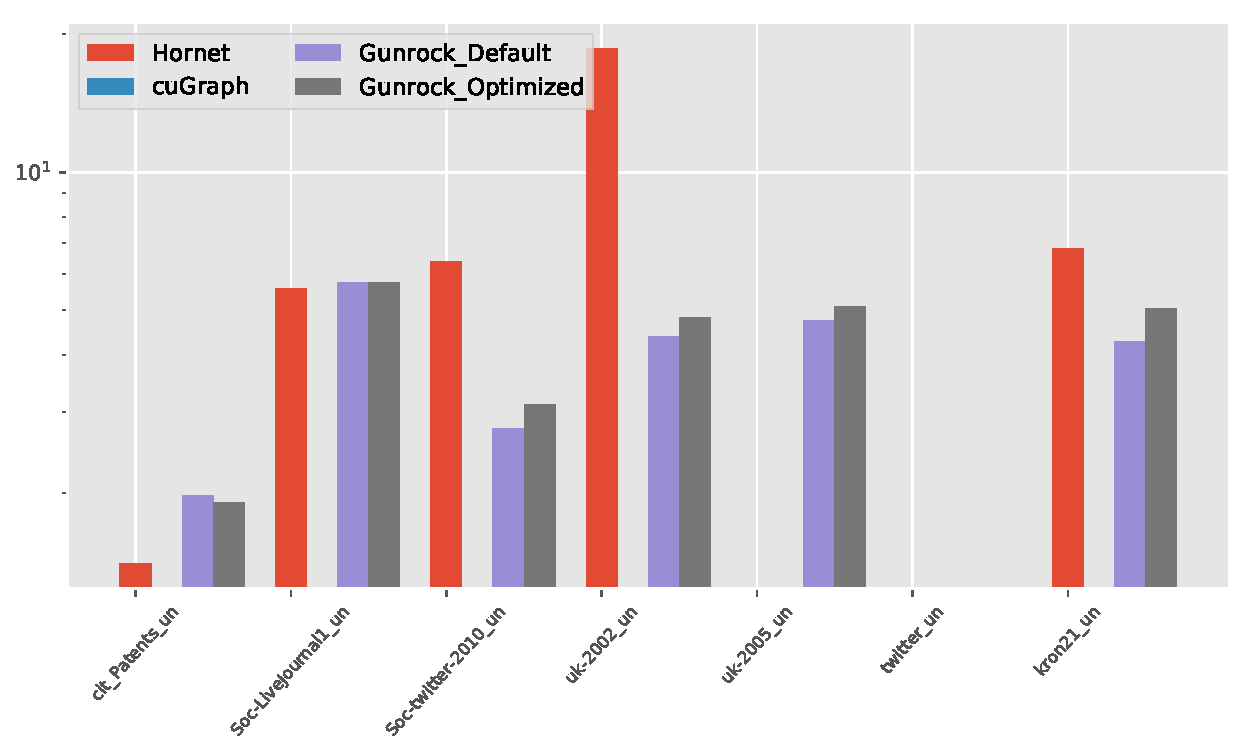
\includegraphics[width=.4\linewidth]{plots/log_GTEPS_G_CC_VS16.pdf}\\[-1ex]
\rowname{(V100-32GB) \small\textbf{CC}}&
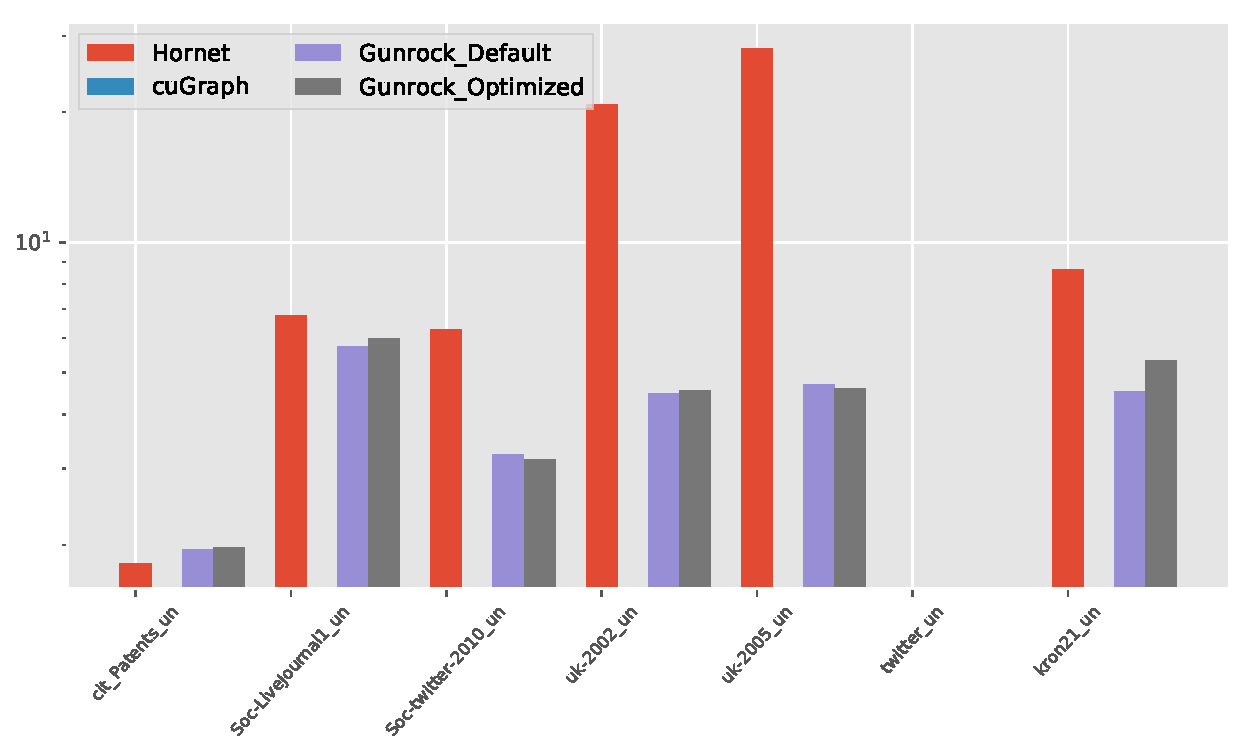
\includegraphics[width=.4\linewidth]{plots/log_GTEPS_G_CC_VP32.pdf}&
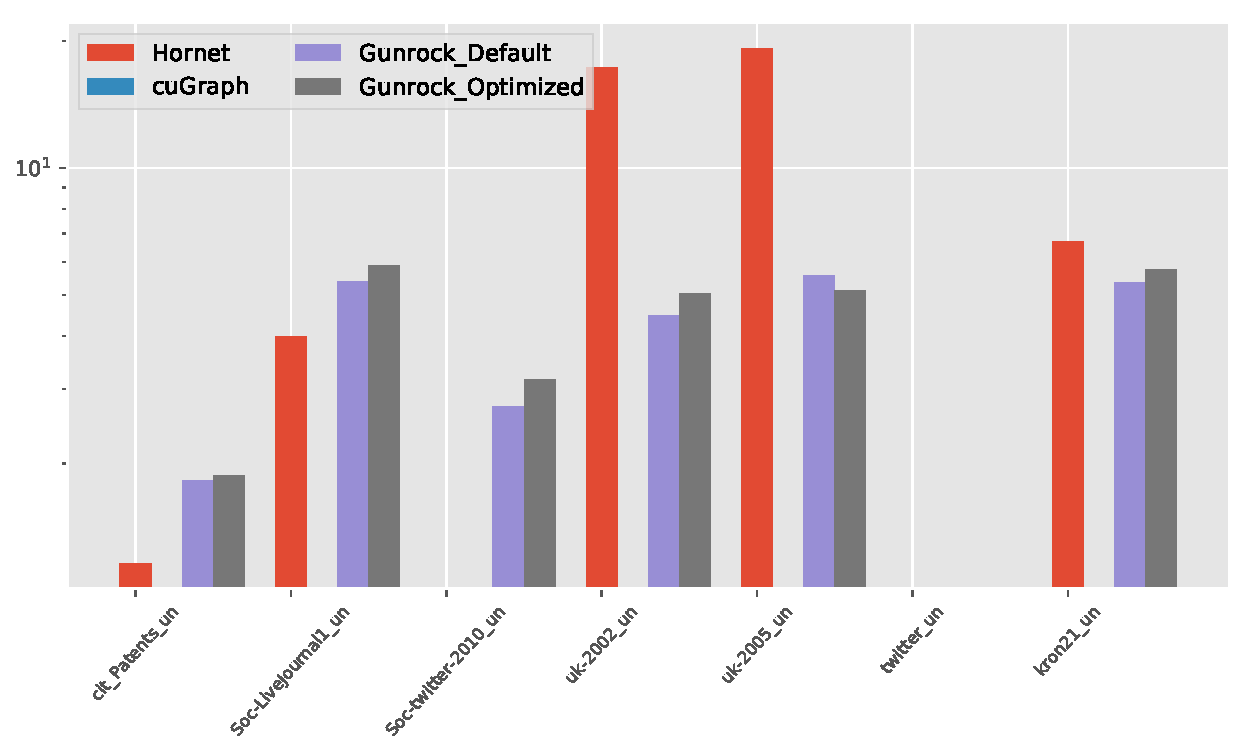
\includegraphics[width=.4\linewidth]{plots/log_GTEPS_G_CC_VS32.pdf}\\[-1ex]
\end{tabular}
\caption{[TBD] TC cuGraph results will be added}%
\label{fig:GTEPS_CC}
\end{figure}

We configured the frameworks with appropriate parameters for the functionality we evaluated. For instance, for Gunrock, we obtained results using both tuned and default parallelization options. 

For each case the operating systems, device driver types, and the versions of each are identical. As mentioned in \ref{sec:experiment-setup}, performance effects as a result of CPU differences are minimal since the measurement of computation time is only conducted on the GPU side. However, any processor-specific optimizations in the driver might affect performance. Note that the CPU types are different with respect to form factor and cache size; all of these differences are encapsulated in the general interconnect types, \emph{i.e.}, PCI-E and SXM, in the rest of this section.

 \subsection{Breadth First Search}
%[Euna] cuGraph BFS uses BLAS? not traversal?
%[Euna] Gunrock BFS is faster because of direction optimized implementation? refer to "four optimization strategies for graph traversal"
For most cases we found that cuGraph, the only BLAS based implementation, was slower than the vertex-centric implementation. In some cases it was up to $4 \times$ slower than Hornet and $20\times$ slower than Gunrock's faster implementation with parallelization options. Gunrock's BFS utilizes the popular bottom-up BFS scheme which is an algorithmic optimization available for vertex-centric algorithms that is not available for BLAS based implementations.
 
% Hornet's vertex-centric BFS algorithm has comparable performance to Gunrock's default BFS. For Gunrock we also report an optimized execution times where the BFS runtime parameters\footnote{Including the parameters that determine when to swap between the classic top-down and the new bottom-up algorithm} are set to get the best execution for a specific graph. In many cases, these parameters are not known \emph{a priori}, though they do offer an insight on performance gains 
Hornet's vertex-centric BFS algorithm has comparable performance to Gunrock's default BFS. For Gunrock we also report an optimized execution times where the BFS runtime parameters, including the parameters that determine when to swap between the classic top-down and the new bottom-up algorithm, are set to get the best execution for a specific graph. In many cases, these parameters are not known \emph{a priori}, though they do offer an insight on performance gains 
%\marginnote{This is a margin note using the geometry package, set at 5cm vertical offset to the first line it is typeset.}[5cm]
%how much additional performance can be gained 
if these parameters %can be 
selected in advance. In order to fully exploit the Gunrock's BFS performance enhancement, we used optimization parameter for Gunrock as ``--idempotence --queue-sizing=6.5 --in-sizing=4 --iteration-num=10 --direction-optimized --device=0 --traversal-mode=LB\_CULL --do\_a=0.200 --do\_b=0.1''. The details of optimization strategies for graph traversal, as well as their effectiveness and trade-offs are enumerated in \cite{wang2017gunrock}.

The results of our experimentation show that in the BFS case, with respect to SXM versus PCI-E, cuGraph is better when SXM is used, Hornet is better when using a PCI-E form factor, and Gunrock is slightly faster in the PCI-E form factor. Unlike in the Hornet case, the performance difference when using SXM versus PCI-E is not as pronounced with Gunrock. 

With respect to the P100 versus the V100, Hornet's BFS performance is better with the P100; cuGraph's performance is better with the V100; and Gunrock runs faster with the V100 as well. It should also be noted that cuGraph's V100 performance is significantly improved with larger graphs.

From the memory access latency perspective, the best performer was V100 with 16GB among the three systems tested, but some very large graphs, such as the uk-2002 and twitter graphs, could not complete the computation within 16GB. A traversal algorithm like BFS shows different behaviors than other types of algorithms. Other algorithms will be discussed below.

%1)	SXM vs. PCI with BFS: cuGraph good with SXM, Hornet is better with PCI, Gunrock slightly faster in PCI but doesn’t affected as much as Hornet does.
% 2)	SXM vs. PCI with other algorithms
% -	PCI is better: BFS, BC and CC
% -	SXM is better: PR 
% -	In TC case, SXM is better when graphs are big, PCI is better with small graphs
% 3)	P100 vs. V100: Hornet BFS is better with P100, cuGraph is better with V100 (especially when the graphs are bigger), and Gunrock is better with V100.
% 4)	Memory access latency: 16GB system is faster than 32GB system if the memory size can handle the computation; V100 16GB often shows better performance than V100 32GB.
% 5)	 Gurock optimization: very fast with the right optimization parameters. Those parameters can be set depending on the algorithm (although we used almost the same speed up parameter for most of the algorithms), and depending on the graphs as well (c.f. different characteristics of graphs…) 

\subsection{PageRank}
Recall, PageRank algorithms can terminate their execution depending on the convergence requirements, as such we report the average time for each iteration. 
For efficiency, the termination conditions for PageRank are typically set as a maximum number of iterations or a convergence criteria that ensures the gap of PageRank scores between the current iteration and that of previous iteration meet some lower bound. We set the maximum iteration number as 50 for our experiments for all the frameworks. 
Each PageRank implementation in each framework represents this score gap with different names (``threshold'' in Hornet, ``error'' in Gunrock and ``tolerance'' in cuGraph) and have a distinct function of this user algorithmic parameter. The \emph{threshold} for Hornet is the sum of PageRank score gaps in all vertices in the graph while the \emph{error} in Gunrock is used to check each score gap in each vertex. The \emph{tolerance} value in cuGraph is compared to the Euclidean distance of all vertices in the graph. 
Furthermore, those values for the convergence criteria have different behaviors and are set differently in each framework. %Our goal was to set this value to be very small such that the maximal number of iterations will be completed. As such, we normalize the execution time by the number of iterations for each framework.
%[Euna] It didn't go all the way through to the maximum iterations in our test; most of iterations are in the range of 10 to 30
We choose these score gap values as carefully as possible so that they result in generating a similar number of PageRank iterations across all of the frameworks. Note that we are not aiming for the number of iterations to be equal, just close. Because of this, we provide the runtime per each iteration rather than that of the total PageRank computation.

From a performance perspective, the execution times of Hornet and Gunrock are comparable for most graphs, though there are some cases where one of the frameworks is up to $2\times$ faster than the other. This occurs for both frameworks. cuGraph did not finish for a large number of graphs. 


Similar to the BFS results, using the V100 with 16GB produces the best performance in PageRank algorithm. The difference is that the V100 is always faster than the P100, including Hornet. Interestingly, Gunrock optimized parallelization options did not produce a significant difference in runtime unlike in the BFS case. Another interesting finding is that SXM works well with algorithms requiring iterative and intensive computation like PageRank. We found SXM outperformed PCI-E in most frameworks, especially on large graphs. When graphs are big, the amortized cost produces a better performance in SXM.

% 1.	V100 16GB is the winner in most of case
% 2.	SXM works better for most of frameworks
% 3.	Gunrock opt technique doesn’t affect much in PR (comparing to BFS)
% 4.	When graphs are big the amortized cost produces a better performance in SXM
% 5.	V100 is always better in PR (including Hornet)


\subsection{Betweenness Centrality}

For betweenness centrality (BC), we used the root with the largest degree to compare the performance of the frameworks. Gunrock's faster algorithm was in most cases $3\times-4\times$ faster than Hornet. There are a few instances where Hornet is $2\times$ faster than Gunrock. The BFS traversal used in BC is a top-down BFS for both Hornet and Gunrock. We are unable to report BC times for cuGraph as it is currently unsupported.

BC is a traversal algorithm that requires a significant amount of computation. V100 produced the best performance in all three frameworks and V100 with 32GB is the winner in BC unlike PR or BFS, as the memory intensive computations deteriorates the performance of the V100 with 16GB of memory. Similar to the previous results in BFS and PR, SXM can be a good consideration if the size of the graph of interest is bigger than the uk-2005 directed graph. Note that Gunrock's parallelization options are not effective when computing BC.

% 1.	Memory intensive computation deteriorated V100 16GB performance for handing memory management; V100 32GB is the winner in BC unlike PR and BFS
% 2.	Similarly, SXM can be a good consideration if the graphs of interests are bigger than uk-2005 directed
% 3.	V100 is faster than P100 in BC, including hornet
% 4.	Gunrock opt effect is not huge with BC

\subsection{Connected Components}

Hornet and Gunrock have two very distinct implementations of connected components. Gunrock uses a label propagation approach that is an extension of the popular \cite{ShiloachVishkin} algorithm. In contrast, Hornet uses a BFS based implementation that finds all the vertices that are connected to a given root. Hornet then iterates over the vertices to find vertices that are not part of a connect component. %This explains the lar
%[Euna] This explains the lar... the sentence is not finished.
%[Euna] V100 SXM 32GB data is not collected yet
We are unable to report times for cuGraph as it is currently does not support connected components.

Since Hornet and Gunrock run distinct connected component algorithms, as a result, they return sets of different CCs. Thus, direct comparison of their runtimes do not show the capabilities of the frameworks. Similar to the BFS results, Hornet performs better in systems with a PCI-E form factor while Gunrock produces the better performance in SXM systems. When the graph size is below uk-2005 in the P100 case, V100 is always a better performer with SXM, including with uk-2005. Computation of the twitter case failed in both Gunrock and Hornet. In the V100 32GB case, Gunrock optimization occasionally appears slower than the default Gunrock configuration with the uk-2005 and twitter graphs.

% %1.	V100 SXM 32GB data is not collected yet
% %2.	Need to check which CC algorithm used for Gunrock and Hornet respectively, because the number of communities appears differently.. Simple runtime comparison doesn’t make a sense.
% 3.	Hornet: SXM <<< PCI 
% 4.	Gunrock (default/opt): SXM >>> PCI (when the graph size is below uk2005 in P100, V100 is always better with SXM including uk2005. Twitter computation failed both Gunrock and Hornet)
% 5.	cuGraph doesn’t support CC
% 6.	V100 32GB: Gunrock opt sometimes appears slower than def with uk2005 and twitter graphs.



\subsection{Triangle Counting}
%[Euna] cuGraph TC should be added
%[Euna] V100 SXM 32GB data is not collected yet

[TBD] Triangle Counting (TC) is currently only available in the Hornet framework. The SXM form factor shows better performance than PCI-E; the difference is greater in P100 than V100. The V100 produces almost $2\times$ speed up in TC than P100.

% 1.	Only Hornet
% 2.	SXM vs. PCI: SXM is better, especially the difference appears bigger in P100 than V100
% 3.	V100 SXM 32GB data is not collected yet
% 4.	P100 <<<<< V100 (almost 2x speed up)

\paragraph{Each Framework}
There are occasionally outlying cases, but in general Gunrock with parallelization options produces the best performance among the three frameworks. Gunrock default shows similar results with Hornet in many cases, while cuGraphs shows the slowest runtime and largest memory usage in most of benchmarks.

\paragraph{PCI-E Vs. SXM Form Factor}
As part of our extensive benchmarking, the algorithms were executed on a wide range of GPUs, including identical GPUs that came in different form factors. For Gunrock, we typically see the performance increase when moving from the PCI-E version of the GPU to its respective SXM form factor (which has better performance and a higher frequency). In contrast this was not the case for traversal algorithms in Hornet, especially for smaller graphs. For larger graphs, Hornet obtained  better performance with the SXM form factor with computationally intensive algorithms.

Specifically, Hornet executes a large number of simple GPU kernels as part of its load-balancing whereas, Gunrock executes fewer and more elaborate kernels. While the performance of SXM cards is typically higher than its PCI-E counterpart, it seems that GPU kernel launch is higher for SXM GPUs. Therefore, on the SXM cards, running a larger number of simple kernels introduces a greater overhead. Thus, it seems that it might be desirable to design a load-balancing that requires fewer GPU kernel launches. This is why SXM produces better performance in general in heavy computations on larger graphs due to its amortized launch cost.